% Options for packages loaded elsewhere
\PassOptionsToPackage{unicode}{hyperref}
\PassOptionsToPackage{hyphens}{url}
%
\documentclass[
]{article}
\usepackage{lmodern}
\usepackage{amssymb,amsmath}
\usepackage{ifxetex,ifluatex}
\ifnum 0\ifxetex 1\fi\ifluatex 1\fi=0 % if pdftex
  \usepackage[T1]{fontenc}
  \usepackage[utf8]{inputenc}
  \usepackage{textcomp} % provide euro and other symbols
\else % if luatex or xetex
  \usepackage{unicode-math}
  \defaultfontfeatures{Scale=MatchLowercase}
  \defaultfontfeatures[\rmfamily]{Ligatures=TeX,Scale=1}
\fi
% Use upquote if available, for straight quotes in verbatim environments
\IfFileExists{upquote.sty}{\usepackage{upquote}}{}
\IfFileExists{microtype.sty}{% use microtype if available
  \usepackage[]{microtype}
  \UseMicrotypeSet[protrusion]{basicmath} % disable protrusion for tt fonts
}{}
\makeatletter
\@ifundefined{KOMAClassName}{% if non-KOMA class
  \IfFileExists{parskip.sty}{%
    \usepackage{parskip}
  }{% else
    \setlength{\parindent}{0pt}
    \setlength{\parskip}{6pt plus 2pt minus 1pt}}
}{% if KOMA class
  \KOMAoptions{parskip=half}}
\makeatother
\usepackage{xcolor}
\IfFileExists{xurl.sty}{\usepackage{xurl}}{} % add URL line breaks if available
\IfFileExists{bookmark.sty}{\usepackage{bookmark}}{\usepackage{hyperref}}
\hypersetup{
  pdftitle={Power Under Multiplicity Project (PUMP): Estimating Power, Minimum Detectable Effect Size and Sample Size When Adjusting for Multiple Outcomes},
  hidelinks,
  pdfcreator={LaTeX via pandoc}}
\urlstyle{same} % disable monospaced font for URLs
\usepackage[margin=1in]{geometry}
\usepackage{color}
\usepackage{fancyvrb}
\newcommand{\VerbBar}{|}
\newcommand{\VERB}{\Verb[commandchars=\\\{\}]}
\DefineVerbatimEnvironment{Highlighting}{Verbatim}{commandchars=\\\{\}}
% Add ',fontsize=\small' for more characters per line
\usepackage{framed}
\definecolor{shadecolor}{RGB}{248,248,248}
\newenvironment{Shaded}{\begin{snugshade}}{\end{snugshade}}
\newcommand{\AlertTok}[1]{\textcolor[rgb]{0.94,0.16,0.16}{#1}}
\newcommand{\AnnotationTok}[1]{\textcolor[rgb]{0.56,0.35,0.01}{\textbf{\textit{#1}}}}
\newcommand{\AttributeTok}[1]{\textcolor[rgb]{0.77,0.63,0.00}{#1}}
\newcommand{\BaseNTok}[1]{\textcolor[rgb]{0.00,0.00,0.81}{#1}}
\newcommand{\BuiltInTok}[1]{#1}
\newcommand{\CharTok}[1]{\textcolor[rgb]{0.31,0.60,0.02}{#1}}
\newcommand{\CommentTok}[1]{\textcolor[rgb]{0.56,0.35,0.01}{\textit{#1}}}
\newcommand{\CommentVarTok}[1]{\textcolor[rgb]{0.56,0.35,0.01}{\textbf{\textit{#1}}}}
\newcommand{\ConstantTok}[1]{\textcolor[rgb]{0.00,0.00,0.00}{#1}}
\newcommand{\ControlFlowTok}[1]{\textcolor[rgb]{0.13,0.29,0.53}{\textbf{#1}}}
\newcommand{\DataTypeTok}[1]{\textcolor[rgb]{0.13,0.29,0.53}{#1}}
\newcommand{\DecValTok}[1]{\textcolor[rgb]{0.00,0.00,0.81}{#1}}
\newcommand{\DocumentationTok}[1]{\textcolor[rgb]{0.56,0.35,0.01}{\textbf{\textit{#1}}}}
\newcommand{\ErrorTok}[1]{\textcolor[rgb]{0.64,0.00,0.00}{\textbf{#1}}}
\newcommand{\ExtensionTok}[1]{#1}
\newcommand{\FloatTok}[1]{\textcolor[rgb]{0.00,0.00,0.81}{#1}}
\newcommand{\FunctionTok}[1]{\textcolor[rgb]{0.00,0.00,0.00}{#1}}
\newcommand{\ImportTok}[1]{#1}
\newcommand{\InformationTok}[1]{\textcolor[rgb]{0.56,0.35,0.01}{\textbf{\textit{#1}}}}
\newcommand{\KeywordTok}[1]{\textcolor[rgb]{0.13,0.29,0.53}{\textbf{#1}}}
\newcommand{\NormalTok}[1]{#1}
\newcommand{\OperatorTok}[1]{\textcolor[rgb]{0.81,0.36,0.00}{\textbf{#1}}}
\newcommand{\OtherTok}[1]{\textcolor[rgb]{0.56,0.35,0.01}{#1}}
\newcommand{\PreprocessorTok}[1]{\textcolor[rgb]{0.56,0.35,0.01}{\textit{#1}}}
\newcommand{\RegionMarkerTok}[1]{#1}
\newcommand{\SpecialCharTok}[1]{\textcolor[rgb]{0.00,0.00,0.00}{#1}}
\newcommand{\SpecialStringTok}[1]{\textcolor[rgb]{0.31,0.60,0.02}{#1}}
\newcommand{\StringTok}[1]{\textcolor[rgb]{0.31,0.60,0.02}{#1}}
\newcommand{\VariableTok}[1]{\textcolor[rgb]{0.00,0.00,0.00}{#1}}
\newcommand{\VerbatimStringTok}[1]{\textcolor[rgb]{0.31,0.60,0.02}{#1}}
\newcommand{\WarningTok}[1]{\textcolor[rgb]{0.56,0.35,0.01}{\textbf{\textit{#1}}}}
\usepackage{graphicx}
\makeatletter
\def\maxwidth{\ifdim\Gin@nat@width>\linewidth\linewidth\else\Gin@nat@width\fi}
\def\maxheight{\ifdim\Gin@nat@height>\textheight\textheight\else\Gin@nat@height\fi}
\makeatother
% Scale images if necessary, so that they will not overflow the page
% margins by default, and it is still possible to overwrite the defaults
% using explicit options in \includegraphics[width, height, ...]{}
\setkeys{Gin}{width=\maxwidth,height=\maxheight,keepaspectratio}
% Set default figure placement to htbp
\makeatletter
\def\fps@figure{htbp}
\makeatother
\setlength{\emergencystretch}{3em} % prevent overfull lines
\providecommand{\tightlist}{%
  \setlength{\itemsep}{0pt}\setlength{\parskip}{0pt}}
\setcounter{secnumdepth}{5}
\usepackage{setspace}
\usepackage{color}
\usepackage{booktabs}
\usepackage{longtable}
\usepackage{array}
\usepackage{multirow}
\usepackage{wrapfig}
\usepackage{float}
\usepackage{colortbl}
\usepackage{pdflscape}
\usepackage{tabu}
\usepackage{threeparttable}
\usepackage{threeparttablex}
\usepackage[normalem]{ulem}
\usepackage{makecell}
\usepackage{xcolor}
\newlength{\cslhangindent}
\setlength{\cslhangindent}{1.5em}
\newenvironment{cslreferences}%
  {\setlength{\parindent}{0pt}%
  \everypar{\setlength{\hangindent}{\cslhangindent}}\ignorespaces}%
  {\par}

\title{Power Under Multiplicity Project (PUMP): Estimating Power,
Minimum Detectable Effect Size and Sample Size When Adjusting for
Multiple Outcomes}
\author{}
\date{\vspace{-2.5em}}

\begin{document}
\maketitle

\doublespacing

\section*{Abstract}

For randomized controlled trials (RCTs) with a single intervention being
measured on multiple outcomes, researchers often apply a multiple
testing procedure (such as Bonferroni or Benjamini-Hochberg) to adjust
\(p\)-values. Such an adjustment reduces the likelihood of spurious
findings, but also changes the statistical power, sometimes
substantially, which reduces the probability of detecting effects when
they do exist. However, this consideration is frequently ignored in
typical power analyses, as existing tools do not easily accommodate the
use of multiple testing procedures. We introduce the \texttt{PUMP}
\texttt{R} package as a tool for analysts to estimate statistical power,
minimum detectable effect size, and sample size requirements for
multi-level RCTs with multiple outcomes. Multiple outcomes are accounted
for in two ways. First, power estimates from \texttt{PUMP} properly
account for the adjustment in \(p\)-values from applying a multiple
testing procedure. Second, as researchers change their focus from one
outcome to multiple outcomes, different definitions of statistical power
emerge. \texttt{PUMP} allows researchers to consider a variety of
definitions of power, as some may be more appropriate for the goals of
their study. The package estimates power for frequentist multi-level
mixed effects models, and supports a variety of commonly-used RCT
designs and models and multiple testing procedures. In addition to the
main functionality of estimating power, minimum detectable effect size,
and sample size requirements, the package allows the user to easily
explore sensitivity of these quantities to changes in underlying
assumptions.

\section{Introduction}
\label{sec:intro}

The \texttt{PUMP} \texttt{R} package addresses an urgent need among
researchers: an open-source software tool to design multi-level
randomized controlled trials (RCTs) with adequate statistical power.
With this package, researchers can estimate statistical power, minimum
detectable effect size (MDES), and needed sample size for multi-level
experimental designs, in which units are nested within hierarchical
structures such as students nested within schools nested within school
districts. The statistical power is calculated for estimating the impact
of a single intervention on multiple outcomes. The package uses a
frequentist framework of mixed effects regression models, which is
currently the prevailing framework for estimating impacts from
experiments in education and other social policy
research.\footnote{Other options include nonparametric or Bayesian methods, but these are less prevalent in applied research (for example, see @GELMANETAL2012, @GelmanHill2007).}

To our knowledge, none of the existing software tools for power
calculations allow researchers to account for multiple hypothesis tests
and the use of a multiple testing procedure (MTP). MTPs adjust
\(p\)-values to reduce the likelihood of spurious findings when
researchers are testing for effects on multiple outcomes. This
adjustment can result in a substantial change in statistical power,
greatly reducing the probability of detecting effects when they do
exist. Unfortunately, when designing studies, researchers who plan to
test for effects on multiple outcomes and employ MTPs frequently ignore
the power implications of the MTPs.

Also, as researchers change their focus from one outcome to multiple
outcomes, multiple definitions of statistical power emerge (Chen (2011);
Dudoit (2003); Senn and Bretz (2007); Westfall and Wolfinger (2011)).
The \texttt{PUMP} package allows researchers to consider multiple
definitions of power, as some may be most suited for the goals of their
study. The definitions of power include:

\begin{itemize}
\tightlist
\item
  \textbf{individual power}: the probability of detecting an effect of a
  particular size (specified by the researcher) or larger for each
  hypothesis test. Individual power corresponds to how power is defined
  when there is focus on a single outcome.
\item
  \textbf{\(1-\)minimal power}: the probability of detecting effects of
  at least a particular size on at least one outcome. Similarly, the
  researcher can consider \textbf{\(d-\)minimal power} for any \(d\)
  less than the number of outcomes, or fractional powers, such as
  \(1/2-\)minimal power.
\item
  \textbf{complete power}: the power to detect effects of at least a
  particular size on \emph{all} outcomes.
\end{itemize}

The prevailing default in many studies---individual power---may or may
not be the most appropriate type of power. If the researcher's goal is
to find statistically significant estimates of effects on most or all
primary outcomes of interest, then their power may be much lower than
anticipated when multiplicity adjustments are taken into account. On the
other hand, if the researcher's goal is to find statistically
significant estimates of effects on at least one or a small proportion
of outcomes, their power may be much better than anticipated. In both of
these cases, by not accounting for both the challenges and opportunities
arising from multiple outcomes, a researcher may find they have wasted
resources, either by designing an underpowered study that cannot detect
the desired effect sizes, or by designing an overpowered study that had
a larger sample size than necessary. We introduce the \texttt{PUMP}
package to allow for directly answering questions that take multiple
outcomes into account, such as:

\begin{itemize}
\tightlist
\item
  How many schools would I need to detect a given effect on at least
  three of my five outcomes?
\item
  What size effect can I reliably detect on each outcome, given a
  planned MTP across all my outcomes?
\item
  How would the power to detect a given effect change if only half my
  outcomes truly had impact?
\end{itemize}

The methods in the PUMP package build on those introduced in Porter
(2018). This earlier paper focused only on a single RCT design and model
--- a multisite RCT with the blocked randomization of individuals, in
which effects are estimated using a model with block-specific intercepts
and with the assumption of constant effects across all units. This
earlier paper also did not produce software to assist researchers in
implementing its methods. With this current paper and with the
introduction of the PUMP package, we extend the methodology to nine
additional multi-level RCT designs and models. Also, while Porter (2018)
focused on estimates of power, PUMP goes further to also estimate MDES
and sample size requirements that take multiplicity adjustments into
account.

\texttt{PUMP} extends functionality of the popular PowerUp! \texttt{R}
package (and related tools in the form of a spreadsheet and Shiny
application), which compute power or MDES for multi-level RCTs with a
single outcome (Dong and Maynard (2013)). For a wide variety of RCT
designs with a single outcome, researchers can take advantage of
closed-form solutions and numerous power estimation tools. For example,
in education and social policy research, see Dong and Maynard (2013);
Hedges and Rhoads (2010); Raudenbush et al. (2011); Spybrook et al.
(2011). However, closed-form solutions are difficult or impossible to
derive when an MTP is applied to a setting with multiple outcomes.
Instead, we use a simulation-based approach to achieve estimates of
power.

In order to calculate power, the researcher specifies information about
the sample size at each level, the minimum detectable effect size for
each outcome (the smallest true effect sizes to detect with statistical
significance, in units of standard deviations), the level of statistical
significance, and parameters of the data generating distribution. An
``effect size'' generally refers to the standardized mean difference
effect size, which ``equals the difference in mean outcomes for the
treatment group and control group, divided by the standard deviation of
outcomes across subjects within experimental groups'' (Bloom (2006)).
Researchers often use effect sizes to standardize outcomes so that
outcomes with different scales can be directly compared.

The package includes three core functions:

\begin{itemize}
\tightlist
\item
  \texttt{pump\_power()} for calculating power given a experimental
  design and assumed model, parameters, and minimum detectable effect
  size.
\item
  \texttt{pump\_mdes()} for calculating minimum detectable effect size
  given a target power and sample sizes.
\item
  \texttt{pump\_sample()} for calculating the required sample size for
  achieving a given target power for a given minimum detectable effect
  size.
\end{itemize}

For any of these core functions, the user begins with two main choices.
First, the user chooses the assumed design and model of the RCT. The
\texttt{PUMP} package covers a range of multi-level designs, up to 3
levels of hierarchy, that researchers typically use in practice, in
which research units are nested in hierarchical groups. Our power
calculations assume the user will be analyzing these RCTs using
frequentist mixed-effects regression models, containing a combination of
fixed or random intercepts and treatment impacts at different levels, as
we explain in detail in Section\textasciitilde{}\ref{sec:est_power} and
in the Supplementary Materials. Second, the user chooses the MTP to be
applied. \texttt{PUMP} supports 5 common MTPs --- Bonferroni, Holm,
single-step and step-down versions of Westfall-Young, and
Benjamini-Hochberg. After these two main choices, the user must also
make a variety of decisions about parameters of the data generating
distribution.

The package also includes functions that allow users to easily explore
power over a range of possible values of parameters. This exploration
encourages the user to determine the sensitivity of estimates to
different assumptions. \texttt{PUMP} also visually displays results.
These additional functions include:

\begin{itemize}
\tightlist
\item
  \texttt{pump\_power\_grid()}, \texttt{pump\_mdes\_grid()}, and
  \texttt{pump\_sample\_grid()} for calculating the given output over a
  range of possible parameter values.
\item
  \texttt{update()} to re-run an existing calculation with a small
  number of parameters updated.
\item
  \texttt{plot()} on any \texttt{PUMP}-generated object to generate
  plots (including grid outputs).
\end{itemize}

The authors of the \texttt{PUMP} package have also created a web
application built with R Shiny. This web application calls the
\texttt{PUMP} package and allows users to conduct calculations with a
user-friendly interface, but it is less flexible than the package, with
a focus on simpler scenarios (e.g., 10 or fewer outcomes). The app can
be found at www.pumpmdrc.io.

The remainder of this paper is organized as follows. In Section
\ref{sec:diplomas}, we introduce Diplomas Now, an educational
experiment, to be used as a running example throughout the paper. We
note, however, that the problem of power estimation for multi-level RCTs
is not exclusive to the educational setting. In Section
\ref{sec:mtp_overview}, we provide a summary of the multiple testing
problem. Also in Section \ref{sec:mtp_overview}, we present an overview
of the statistical challenges introduced by multiple hypothesis testing
and how MTPs protect against spurious impact findings. In Section
\ref{sec:est}, we introduce our methodology for estimating power when
taking the use of MTPs into account. This section also briefly discusses
our validation process. Section\textasciitilde{}\ref{sec:choices}
discusses the various choices a user must make when using the package,
including the designs and models, MTPs, and key design and model
parameters. Section \ref{sec:vignette} provides a detailed presentation
of the \texttt{PUMP} package with multiple examples of using the
packages functions to conduct calculations for our education RCT
example. Section \ref{sec:conclusion} is a brief conclusion.

\section{Diplomas Now}
\label{sec:diplomas}

We illustrate our package using an example of a published RCT that
evaluated a secondary school model called Diplomas Now. The Diplomas Now
model is designed to increase high school graduation rates and
post-secondary readiness. Evaluators conducted a RCT comparing schools
who implemented the model to business-as-usual. We refer to this example
throughout this paper to illustrate key concepts and to illustrate the
application of the \texttt{PUMP} package.

The Diplomas Now model, created by three national organizations, Talent
Development, City Year, and Communities In Schools, targets underfunded
urban middle and high schools with many students who are not performing
well academically. The model is designed to be robust enough to
transform high-poverty and high-needs middle and high schools attended
by many students who fall off the path to high school graduation.
Diplomas Now, with MDRC as a partner, was one of the first validation
grants awarded as part of the Investing in Innovation (i3) competition
administered by the federal Department of Education.

We follow the general design of the Diplomas Now evaluation, conducted
by MDRC. The RCT contains three levels (students within schools within
districts) with random assignment at level 2 (schools). The initial
evaluation, included two cohorts of schools with each cohort
implementing for two years (2011-2013 for Cohort 1 and 2012-2014 for
Cohort 2). The cohorts included 62 secondary schools (both middle and
high schools) in 11 school districts that agreed to participate. Schools
in the active treatment group were assigned to implement the Diplomas
Now model, while the schools in the control group continued their
existing school programs or implemented other reform strategies of their
choosing (Corrin W. (2016).) The MDRC researchers conducted
randomization of the schools within blocks defined by district, school
type, and year of roll-out. After some schools were dropped from the
study due to structural reasons, the researchers were left with 29 high
schools and 29 middle schools grouped in 21 random assignment blocks.
Within each block, schools were randomized to the active treatment or
business-as-usual, resulting in 32 schools in the treatment group, and
30 schools in the control group.

The evaluation focused on three categories of outcomes: Attendance,
Behavior, and Course performance, called the ``ABC's'', with multiple
measures for each category. In addition, the evaluation measured an
overall ABC composite measures of whether a student is above given
thresholds on all three categories. This grouping constitutes 12 total
outcomes of interest. Evaluating each of the 12 outcomes independently
would not be good practice, as the chance of a spurious finding is not
well controlled. The authors of the MDRC report pre-identified three of
these outcomes as \emph{primary} outcomes before the start of the study
in order to reduce the problem of multiple testing. We, by contrast, use
this example to illustrate what could be done if there was uncertainty
as to what should be the primary outcome. In particular, we illustrate
how to conduct a power analysis to plan a study where one uses multiple
testing adjustment, rather than predesignation, to account for the
multiple outcome problem.

There are different guidelines for how to adjust for groupings of
multiple outcomes in education studies. For example, Schochet (2008)
recommends organizing primary outcomes into domains, conducting tests on
composite domain outcomes, and applying multiplicity corrections to
composites across domains. The What Works Clearinghouse applies
multiplicity corrections to findings within the same domain rather than
across different domains. We do not provide recommendations for which
guidelines to follow when investigating impacts on multiple outcomes.
Rather, we address the fact that researchers across many domains are
increasingly applying MTPs and therefore need to correctly estimate
power, MDES and sample size requirements accounting for this choice. In
our example, we elect to do a power analysis separately for each of the
three outcome groups of the ABC outcomes to control family-wise error
rather than overall error. This strategy means we adjust for the number
of outcomes within each group independently. For illustration purposes,
we focus on one outcome group, attendance, which we will assume contains
five separate outcomes.

\section{Overview of multiple testing}
\label{sec:mtp_overview}

Our motivating example illustrates that researchers are often interested
in testing the effectiveness of a single intervention on multiple
outcomes. The resulting multiplicity of statistical hypothesis tests can
lead to spurious findings of
effects.\footnote{Testing the effectiveness of an intervention for multiple subgroups, at multiple points in time, or across multiple treatment groups also results in a multiplicity of statistical hypotheses and can also lead to spurious findings of effects, but this is beyond the scope of this paper.}
Multiple testing procedures (MTPs) counteract this problem by adjusting
\(p\)-values for effect estimates; generally, \(p\)-values are adjusted
upward to require a higher burden of proof. When not using an MTP, the
probability of finding false positives increases, sometimes
dramatically, with the number of tests. When using an MTP, this
probability is reduced.

First, we remind the reader of how raw, or unadjusted, \(p\)-values are
calculated in this setting, before introducing adjustments due to
multiple testing. Consider that a researcher is interested in testing
the impact of an intervention on \(M\) outcomes. In our running example
of the Diplomas Now study, if we had 5 outcomes in the attendance group,
we would have \(M = 5\). We apply a frequentist hypothesis testing
framework, and frame impacts in terms of effect sizes (\(ES\)). For
outcome \(m\), we can test a null hypothesis of no effect,
\(H_{0_m}: ES_m = 0\), against an alternative hypothesis
\(H_{1_m}: ES_m \neq 0\) for a two-sided tests or \(H_{1_m}: ES_m > 0\)
or \(H_{1_m}: ES_m < 0\) for a one-sided test. We can also conduct a
hypothesis test of a certain assumed effect size \(\gamma\), where the
null hypothesis is \(H_{0_m}: ES_m < \gamma\) and the alternative
hypothesis is \(H_{1_m}: ES_m >= \gamma\). A significance test, such as
a two- or one-sided \(t\)-test, would then typically be driven by a test
statistic given by \begin{equation}
t_m = \frac{\widehat{ES}_m}{SE(\hat{ES}_m)},
\end{equation} where \(SE(\hat{ES}_m)\) is the standard error. A raw
\(p\)-value would then be computed as the probability of being at least
as extreme as the one observed, given that the null hypothesis is true.
For a two-sided test, the raw \(p\)-value for test \(m\) is
\(p_m=2*Pr(T_m \geq |t_m|)\). The \texttt{PUMP} package also allows for
either one-sided or two-sided tests, but we proceed assuming two-sided
tests going
forward.\footnote{For a one-sided test, depending on the direction of our alternative hypothesis, the raw $p$-value for test $m$ is computed as $p_m=Pr(T_m \leq t_m)$ or $p_m=Pr(T_m \geq t_m)$.}

When testing a \emph{single} hypothesis under this framework,
researchers typically specify \(\alpha\), the maximum acceptable
probability of making a Type I error. A Type I error is the probability
of erroneously rejecting the null hypothesis when it is true. The
quantity \(\alpha\) is also referred to as the significance level. If
\(\alpha=0.05\), then the null hypothesis is rejected if the \(p\)-value
is less than \(0.05\), and it is concluded that the intervention had an
effect because there is less than a \(5\)\% chance that this finding is
a false positive.

When one tests \emph{multiple} hypotheses under this framework (such
that \(M>1\)) and one conducts a separate test for each of the
hypotheses with \(\alpha=0.05\), there is a \emph{greater} than \(5\%\)
chance of a false positive finding in the study. If the multiple tests
are independent, the probability that at least one of the null
hypothesis tests will be erroneously rejected is
\[1-Pr(\text{none of the null hypotheses will be erroneously rejected}) = 1-(1-\alpha)^M.\]
Therefore, if researchers are estimating effects on 3 outcomes (and if
these outcomes are independent) the probability of at least one false
positive finding is \(1-(1-0.05)^3=0.14\). If the researchers were
instead estimating effects on 5 independent outcomes, the probability of
at least one false positive finding rises to \(0.23\). This Type I error
inflation for independent outcomes demonstrates the crux of the multiple
testing problem. In practice, however, the multiple outcomes are usually
at least somewhat correlated, which makes the test statistics correlated
and reduces the extent of Type I error inflation. Nonetheless, any error
inflation can still make it problematic to draw reliable conclusions
about the existence of effects above a specified size.

\subsection{Using MTPs to protect against spurious impact findings}
\label{sec:mtp_use}

As introduced above, multiple testing procedures (MTPs) adjust
\(p\)-values to counteract the multiple testing
problem.\footnote{Alternatively, MTPs can decrease the critical values for rejecting hypothesis tests. For ease of presentation, this paper focuses only on the approach of adjusting $p$-values.}
We next describe how using a MTP protects against false positives.

Considering multiple outcomes presents both challenges and
opportunities. First, we discuss the impact of MTPs on individual power.
Recall that the power of an individual hypothesis test is the
probability of correctly rejecting a null hypothesis when the effect is
at least a specified size. We refer to a setting in which the true
impact is at least as large as the desired effect size as a ``false
null'' hypothesis, while a ``true null'' is a setting in which the true
impact is less than the desired effect size. In the proceeding
explanations, when we refer to rejecting a null hypothesis or detecting
an effect, we assume that we are detecting an effect of a certain
pre-specified size. If \(p\)-values are adjusted upward, one is less
likely to reject true nulls, which reduces the probability of Type I
errors, or false positive findings. At the same time, MTPs increase the
probability of a Type II error, or false negative findings, when the
test fails to reject a false null. Individual power is
\(1 - Pr(\text{Type II error})\), so MTPs have the tradeoff of reducing
Type I errors but also reducing individual power.

Next, we consider the impact of multiple outcomes on other definitions
of power. Applying an MTP reduces power according to all definitions of
power relative to the case when no MTP is applied to adjust
\(p\)-values. However, as discussed previously, having multiple outcomes
also allows for a wider variety of definitions of success. Recall that
\(1-\)minimal power is the probability of detecting an effect on at
least one outcome. Typically, \(1-\)minimal power, even after applying a
MTP, is higher than individual power for a hypothesis test on a single,
pre-specified outcome. Depending on the setting, other definitions of
power, such as \(1/2\) or \(1/3\)-minimal power, may or may not have
higher power than the power of a single hypothesis test.

The MTPs that are the focus of this paper have three key features that
affect statistical power: (1) whether the MTP is a familywise procedure
or a false discovery rate procedure; (2) whether the MTP is single-step
or stepwise; and (3) whether the MTP takes the correlation between test
statistics into account. Below we explain each of these features of MTPs
and provide discussion of the new parameter specifications they require
when estimating power.

\subsection{Familywise error rate vs. false discovery error rate}

Familywise procedures reframe Type I error as a rate across the entire
set or ``family'' of multiple hypothesis tests. This rate is called the
familywise error rate (FWER; Tukey (1953)). The FWER is typically set to
the same value as the probability of a Type I error for a single test,
e.g., \(\alpha\). MTPs that control the FWER at \(5\%\) adjust
\(p\)-values in a way that ensures that the probability of at least one
Type I error across the entire set of hypothesis tests is no more than
\(5\%\). The MTPs introduced by Bonferroni (Dunn (1959), Dunn (1961)),
Holm (1979), and Westfall and Young (1993) control the FWER.

MTPs that control false discovery rate (FDR) take an entirely different
approach to the multiple testing problem. FDR is a less stringent
criteria than FWER. Introduced by Benjamini (1995), the FDR is the
expected proportion of all rejected hypotheses that are erroneously
rejected. The two-by-two representation in
Table\textasciitilde{}\ref{tab:twobytwo} is often found in articles on
multiple hypothesis testing, and helps to illustrate the difference
between FWER and FDR. Let \(M\) be the total number of tests. Therefore,
we have \(M\) unobserved truths: whether or not each null hypothesis is
true or false. We also have \(M\) observed decisions: whether or not the
null hypotheses were rejected, because the \(p\)-values were less than
\(\alpha\). In Table\textasciitilde{}\ref{tab:twobytwo}, \(U\), \(V\),
\(W\), and \(X\) are four possible scenarios: the numbers of true or
false hypotheses not rejected or rejected. \(M_0\) and \(M_1\) are the
unobservable numbers of true null and false null hypotheses. \(R\) is
the number of null hypotheses that were rejected, and \(M - R\) is the
number of null hypotheses that were not rejected.

\begin{table}[h!]
\centering
\begin{tabular}{l l l l}
                                      & \multicolumn{3}{c}{Observed decisions}\\ \hline
Unobserved truths                     & Number not rejected     & Number rejected   & Total \\ \hline
Number of true null hypotheses        & $U$                     & $V$               & $M_0$ \\
Number of false null hypotheses       & $W$                     & $X$               & $M_1$ \\ \hline
Total                                 & $M-R$                   & $R$               & $M$
\end{tabular}
\caption{Numbers of hypothesis types and decisions.}
  \label{tab:twobytwo}
\end{table}

In Table\textasciitilde{}\ref{tab:twobytwo}, \(V\) is the number of
erroneously rejected null hypotheses, or the number of false positive
findings. Therefore, the FWER is equivalent to \(Pr(V > 0)\), the
probability of at least one false positive finding. Recall that Type I
error is inflated when testing for effects when no MTPs are applied.
Consider the setting when all the outcomes are independent of each
other. The Type I error is almost \(10\%\) when testing effects on two
independent outcomes and \(23\%\) when testing effects on five
independent outcomes. These Type I error rates both correspond to the
FWER. The goal of MTPs that control the FWER is to bring these
percentages back down to \(5\%\).

Also in Table\textasciitilde{}\ref{tab:twobytwo}, the FDR is equal to
\(E(V/R)\) but is defined to be \(0\) when \(R=0\), or when no
hypotheses are rejected. As is frequently noted in the literature (e.g.,
Shaffer (1995); Schochet (2008)), the FWER and FDR have different
objectives. Control of the FWER protects researchers from spurious
findings and so may be preferred when even a single false positive could
lead to the wrong conclusion about the effectiveness of an intervention.
On the other hand, the FDR is more lenient with false positives.
Researchers may be willing to accept a few false positives, \(V\), when
the total number of rejected hypotheses, \(R\), is large. Note that
under the complete null hypothesis that all \(M\) null hypotheses are
true, the FDR is equal to the FWER. Referring back to
Table\textasciitilde{}\ref{tab:twobytwo}, under the complete null we
have \(V = R\), so \begin{align*}
FDR &= E\left(\frac{V}{R}\right)\\
&=  E\left(\frac{V}{R}\mid R = 0\right) Pr(R = 0) + E\left(\frac{V}{R} \mid R > 0\right)Pr(R > 0) \\
&= 0 \times Pr(R = 0) + 1 \times Pr(R > 0) \\
&= Pr(R > 0) = FWER
\end{align*} However, if any effects truly exist, then
\(FWER \geq FDR\). As a result of the difference in objective between
FWER and FDR, in the case where there is at least one false null
hypothesis (at least one true effect), an MTP that controls the FDR at
\(5\%\) will have a Type I error rate that is greater than \(5\%\).

MTPs may provide either ``weak'' or ``strong'' control of the error rate
they target. An MTP provides ``weak control'' of the FWER or the FDR at
level \(\alpha\) if the control can only be guaranteed when all null
hypotheses are true, e.g.~when the effects on all outcomes are zero. An
MTP provides ``strong control'' of the FWER or FDR at level \(\alpha\)
if the control is guaranteed when some null hypotheses are true and some
are false, e.g.~when there may be effects on at least some outcomes. Of
course, strong control is
preferred.\footnote{The single-step and step-down Westfall Young MTPs (which we discuss below) always provide at least weak control of the FWER. In order for these procedures to provide strong control of the FWER, they require the assumption of subset pivotality (@RN33093).The distribution of the unadjusted test statistics or $p$-values is said to have subset pivotality if for any subset of null hypotheses, the joint distribution of the test statistics or of the $p-$values for the subset is identical to the distribution under the complete null.
A consequence of this assumption is that the permutation of test statistics or $p$-values can be done under the complete null hypothesis rather than under the unknown partial hypothesis (@RN33093).}

\subsection{Single-step vs. stepwise procedures}
\label{sec:stepwise}

A second feature of a MTP that affects its statistical power is whether
it is a ``single-step'' or ``stepwise'' procedure. Single-step
procedures adjust each \(p\)-value independently of the other
\(p\)-values. For example, the Bonferroni MTP multiplies all raw
\(p\)-values by \(M\). Therefore, one \(p\)-value adjustment does not
depend on other \(p\)-value adjustments, only on the number of tests. In
contrast, stepwise procedures first order raw \(p\)-values (or test
statistics), and then adjust according to the order of the tests. The
adjustments depend on the null hypotheses already rejected in previous
steps. For example, the Holm MTP --- the stepwise counterpart to the
Bonferroni MTP --- orders raw \(p\)-values from smallest to largest. The
procedure then multiplies the smallest \(p\)-value by \(M\), the second
smallest \(p\)-value by \(M-1\), and so on. The Holm MTP, like most
other stepwise procedures, also enforces monotonicity: each adjusted
\(p\)-value is greater than or equal to the previous adjusted
\(p\)-value, and enforces that any \(p\)-values is not greater than one.
Overall, stepwise MTPs allow for less adjustment than single-step MTPs
in later steps, and therefore preserve more power (for outcomes in the
later steps). The Bonferroni and Westfall-Young single-step procedure
are single-step; the Holm and Benjamini-Hochberg MTPs and the
Westfall-Young step-down procedure are stepwise. Note that stepwise
procedures may be ``step-down'' or ``step-up,'' referring to whether a
procedure begins with the smallest \(p\)-value, and thus the largest
effect size (step-down) or the largest \(p\)-value (step-up).

Due to the dependencies of adjustments in stepwise MTPs, a new
assumption must be considered when estimating power under multiplicity:
the proportion of outcomes on which there are truly impacts, or,
equivalently, the number of false null hypotheses. Researchers may be
inclined to assume that there will be effects on all outcomes, as
hypotheses of effects probably drive the selection of outcomes in the
first place. However, if the researchers are incorrect, the probability
of detecting the extant effects can be diminished, sometimes
substantially.

\textcolor{red}{Evan found this paragraph a little confusing.  I tried to do some re-working, but would also be happy for someone to tackle a rewrite.}
It is important to point out that under the assumption that some effects
are truly null, we must change our notion of power for \(d-\)minimal
powers (e.g., \(1-\)minimal power, \(1/3-\)minimal power, etc.) and
complete power. While individual power is defined based on the
probability of correctly rejecting false nulls, the definition is
loosened here and includes the probability of erroneous rejections of
true nulls. For example, \(1/3-\)minimal power is defined as the
probability of detecting effects on at least \(1/3\) of the \emph{total
outcomes \(M\)}, regardless of the number of outcomes with true effects.
That is, \(1/3-\)minimal power is not defined as the probability of
detecting effects among the \(M\) outcomes on which the effects truly
exist. This reframing of power is necessary for power to be consistent.
If \(d-\)minimal power were defined based on false nulls, then the value
and interpretation would change depending on what assumption the
researcher is making about the number of false nulls, which is an
unknown quantity. For example, with \(M = 5\) outcomes, the probability
of detecting at least one effect would be very different depending on if
we assume all five outcomes are false nulls, or if we assume only two of
them are false nulls. Complete power, which is the probability of
detecting effects on all outcomes, has similar issues. We define
complete power only in the context where all effects are assumed to be
false nulls --- if any outcomes are assumed to be true nulls, then
complete power is undefined.

There is an additional technical note about the calculation of complete
power.\footnote{Complete power has also been referred to as “conjunctive power” (@RN33091) and “all pairs power” (@RN33097).}
To calculate complete power, we do not need to adjust the \(p\)-values,
and can instead reject each individual test based on the unadjusted
\(p\)-values.\footnote{
Complete power is the power of the omnibus test constructed by whether or not we reject all the null hypotheses.
This test was originally introduced as the intersection-union test because the null hypothesis is expressed as a union and the alternative hypothesis is expressed as an intersection (@Berger1982, @Berger1996).
@Berger1982 showed that if all the individual tests are level $\alpha$, the intersection-union test is also a level $\alpha$ test.
To provide some intuition, we do not need to adjust $p$-values for complete power because it is a special case where  we must reject *all* the hypothesis tests.
Thus, there is no way for the omnibus test to be rejected by chance because of a favorable configuration (@RN23882). 
For example, consider if we have 4 tests, with 2 false nulls and 2 true nulls.
If we consider $3-$minimal power, we just need one of the two true nulls to be rejected by chance alone, and there are two ways for this to occur.
For complete power, there is only one way for us to reject all of the nulls.
The downside of an intersection-union test is that it is conservative: the FWER is generally less than $\alpha$. 
For example, if we have two independent tests with Type I error $\alpha$, then if both of are true nulls, the probability of a Type I error for the omnibus test (the probability of rejecting both null hypotheses) is $\alpha^2$ (@Deng2008).}

\subsection{Correlation between test statistics}
\label{sec:corr}

Finally, a third feature of an MTP that affects its statistical power is
whether or not it takes into account the correlation between test
statistics. The Bonferroni and Holm procedures strongly control the FWER
in all cases, even when the test statistics are correlated, but they
adjust \(p\)-values more than is necessary in that case. Along with the
Bonferroni and Holm MTPs, the Benjamin-Hochberg MTP also does not take
correlations into
account.\footnote{The Benjamini-Hochberg procedure was originally shown to control the FDR for independent test statistics. However, @BenjaminiYekutieli2001 showed that it also controls the FDR for true null hypotheses with “positive regression dependence.” This condition is satisfied
for most applications in practice.} In contrast, both of the
Westfall-Young MTPs rely on the estimation of the joint distribution of
test statistics when the complete null hypothesis (that there are not
effects on any of the outcomes) is true. This joint distribution of the
test statistics is estimated from the study's data. For example, random
permutations of the treatment indicator break the association between
treatment status and outcome. Repeating these permutations a large
number of times, results in a distribution of test statistics under the
complete null. Because the actual data are used to generate this null
distribution, correlations among the test statistics are captured. Then
observed test statistics can be compared with the distribution of test
statistics under the complete null
hypothesis.\footnote{Instead of using test statistics, the Westfall-Young MTPs can alternatively compare raw $p$-values with the estimated joint null distribution of $p$-values.}

\textcolor{red}{KH Note: I am not editing this paragraph in case we rewrite it with correlation tool.}
The correlation between test statistics is a parameter a researcher must
specify in order to estimate power, MDES or sample size requirements
when using an MTP. The \(M\) pairwise correlations are equal to the
\(M\) pairwise correlations between the residuals in the \(M\) impact
models. If there are no covariates in the impact models or if the
\(R^2\)'s of the covariates are equivalent in all impact models, then
the correlations between the test statistics are equal to the
correlations between the outcomes. However, having different \(R^2\)'s
across the impact models reduces the correlations between the residuals
and therefore between test
statistics.\footnote{For example, one of the multiple outcomes may have a baseline covariate with a high $R^2$ while another may have a baseline covariate with
a smaller $R^2$. Also, block dummies may explain more variation in some outcomes than in others.}
Models of outcomes that are highly correlated are more likely to have
residuals that are highly correlated because baseline covariates will
tend to have similar \(R^2\)'s. The gaps between the correlations
between outcomes and the correlations between residuals --- and
therefore the test statistics --- may be wider for moderately or weakly
correlated outcomes. In any case, the upper bounds of correlations
between the test statistics are the correlations between the outcomes.

\section{Estimating power, MDES and sample size in studies with multiple outcomes}
\label{sec:est}

\subsection{Power estimation approach}
\label{sec:est_power}

We take an innovative simulation-based approach to estimating power, as
introduced in Porter (2018). This approach is then also applied to
estimate MDES and sample size. In order to estimate power for a single
outcome, we can often use closed-form algebraic expressions, which are
derived from the assumed model. However, with multiple outcomes, finding
such expressions can be quite difficult, or even impossible. In cases
where it is possible to find a closed-form expression, we would need to
find expressions for every design and model, MTP, and definition of
power. Importantly, we would \emph{also} need to find new expressions
for any possible number of outcomes, which quickly becomes an
intractable problem. Furthermore, in some cases, such as
permutation-based procedures like Westfall-Young approaches, a
closed-form solution does not exist. To avoid these complexities, we
rely on simulation to calculate estimated power. The approach outlined
below can estimate power for any scenario.

If we were to rely on a \emph{full} simulation approach, we could use
the following method to estimate power. We note that we introduce this
full simulation approach to provide intuition, but use a simplified and
less computationally intensive approach in the package, as discussed
below.

\begin{enumerate}
\def\labelenumi{\arabic{enumi}.}
\item
  \emph{Simulate a data sample according to the joint alternative
  hypothesis.} First, we formulate what we will refer to as the
  \emph{joint alternative hypothesis}, which is the set of outcomes we
  assume to have treatment effects above the desired size. We define
  \(\psi_m\) to be the treatment effect for outcome \(m\), with \(M\)
  total outcomes. If we have \(M = 5\) outcomes, as in the Diplomas Now
  study, one possible joint alternative hypothesis is that all outcomes
  have effects above specified sizes:
  \(H_A: \psi_1 > 0.125, \psi_2 > 0.2, \psi_3 > 0.1, \psi_4 > 0.1, \psi_5 > 0.05\).
  Another possible joint alternative hypothesis is one where only the
  first two outcomes have effects above the desired sizes:
  \(H_A: \psi_1 > 0.125, \psi_2 > 0.2, \psi_3 = \psi_4 = \psi_5 = 0\).
  Once our joint alternative hypothesis is specified, we would generate
  simulated data under this hypothesis. To simulate data, we need to
  specify the full set of parameters as mentioned in
  Section\textasciitilde{}\ref{sec:params} that allow for data
  generation. The Supplementary Material contains more details about the
  assumed data-generating process. For example, for the Diplomas Now
  experiment, we would assume a specific data generating process to
  allow us to simulate synthetic students, schools, and districts,
  including covariates, outcomes, and treatment assignment. This process
  would involve specifying parameter values such as \(R^2\), the amount
  of outcome variation explained by covariates at a particular level,
  and translating these parameter choices into data-generating
  parameters, such as the coefficient values for covariates in a linear
  model.
\item
  \emph{Estimate impacts on the simulated data.} Given simulated data,
  we could fit \(M\) regression models (specified to match the
  experimental design and model assumptions). For the models supported
  by \texttt{PUMP}, the relevant functions would be \texttt{lm()},
  \texttt{lmer()} from the \texttt{lme4} library (Bates et al. (2015)),
  and \texttt{interacted\_linear\_estimators()} from the \texttt{blkvar}
  library.\footnote{This package is currently under development on GitHub; see https://github.com/lmiratrix/blkvar}
  From the model output we extract the test statistics \(t_m\) for the
  estimated impacts, one statistic for each outcome, along with
  estimated standard errors.
\item
  \emph{Calculate unadjusted \(p\)-values.} The test statistics and
  standard errors would in turn give raw (unadjusted) \(p\)-values. We
  can either calculate these by hand, or use the \(p\)-values routinely
  returned by regression functions. For Diplomas Now we could run a
  regression model of each attendance measure on treatment status and
  student and school covariates, and extract \(p\)-values from the
  regression outputs.
\item
  \emph{Repeat above steps (1 through 3) for a large number of
  iterations.} Denote the number of iterations \texttt{tnum}. Repeating
  steps \(1\)-\(3\) \texttt{tnum} times results in a matrix of
  unadjusted \(p\)-values which we call \(\mathbf{F}\), and is of
  dimension \(tnum \times M\). One row corresponds to one set of
  simulated raw \(p\)-values from regressions for the \(5\) attendance
  outcomes of interest for Diplomas Now.
\item
  \emph{Adjust \(p\)-values.} For each row, corresponding to one
  simulated dataset, the \(M\) raw \(p\)-values corresponding to the
  \(M\) hypothesis tests can be adjusted according to the desired
  multiple testing procedure. This process generates a new matrix
  \(\mathbf{G}\) of adjusted \(p\)-values. For Bonferroni, Holm, and
  Benjamini-Hochberg adjustments, we use the function \texttt{p.adjust}
  in \texttt{R} (found in the \texttt{stats} package). We developed our
  own functions for implementing adjustment using the Westfall-Young
  procedures. One row corresponds to one set of simulated
  \emph{adjusted} \(p\)-values for the \(5\) attendance outcomes of
  interest for Diplomas Now.
\item
  \emph{Calculate hypothesis rejection indicators.} For any MTP, the
  matrix of adjusted \(p\)-values \(\mathbf{G}\) can then be compared
  with a specified value of \(\alpha\) (the default is \(0.05\), but the
  value can be changed by the user). For each row, corresponding to one
  iteration of simulated data, we record whether or not the null
  hypothesis was rejected for each outcome. This process results in a
  new matrix \(\mathbf{H}\), which contains hypothesis rejection
  indicators (still of dimension \(tnum \times M\)). Using
  \(\mathbf{H}\), we can compute all definitions of power.
\item
  \emph{Calculate power.} To compute the different definitions of power:
\end{enumerate}

\begin{itemize}
\item
  \emph{Individual power} for outcome \(m\) is the proportion of the
  \texttt{tnum} rows in which the null hypothesis \(m\) was rejected
  (the mean of column \(m\) of \(\mathbf{H}\)). We would have \(5\)
  different individual power values for Diplomas Now, corresponding to
  each outcome of interest.
\item
  \emph{\(d\)-minimal power} is the proportion of the \(tnum\) rows in
  which at least \(d\) of the \(M\) hypotheses were
  rejected.\footnote{Note that others refer to $1-$minimal power simply as “minimal power” (e.g., @RN33095; @RN23882; @MTSAS), “disjunctive power” (e.g., @RN33091), or “any pair” power (@RN33097). @RN23882 use the terminology of “r-power” for what is referred to here as $d-$minimal power for d>1.}
  For Diplomas Now, we could consider \(1\)-minimal power through
  \(4\)-minimal power.
\item
  \emph{Complete power} is the proportion of the \(tnum\) rows in which
  all of the null hypotheses were rejected based on the raw \(p\)-values
  rather than adjusted \(p\)-values (based on the matrix \(\mathbf{G}\)
  rather than \(\mathbf{H}\).) We would be interested in complete power
  if we want to evaluate whether Diplomas Now resulted in improvement
  for every single attendance outcome of interest. With \(5\) outcomes,
  this criteria is a relatively strict indicator of success.
\end{itemize}

Above, we outlined a full simulation-based approach for calculating
power. This approach would be computationally intensive because of the
need to generate and analyze a full simulated dataset at each iteration.
We can simplify this process by skipping the simulation of data and
modeling steps. Given an assumed model and correlation structure for the
test statistics, we can directly sample from \(f(t_1, \dots, t_M)\), the
joint alternative distribution of the test statistics. This shortcut
vastly improves both the simplicity and the speed of computation. In
summary, our approach is:

\begin{enumerate}
\def\labelenumi{\arabic{enumi}.}
\tightlist
\item
  \textbf{Generate} draws of \emph{test statistics \(t_1, \dots, t_M\)
  under the joint alternative hypothesis.} This step produces a
  \(tnum \times M\) matrix \(\mathbf{E}\).
\item
  \emph{Calculate unadjusted \(p\)-values.} This produces the matrix
  \(\mathbf{F}\), as in the procedure above.
\item
  \emph{Adjust \(p\)-values.} This produces the matrix \(\mathbf{G}\),
  as in the procedure above.
\item
  \emph{Calculate hypothesis rejection indicators.} This produces the
  matrix \(\mathbf{H}\), as in the procedure above.
\item
  \emph{Calculate power.}
\end{enumerate}

We now describe how to sample from \(f(t_1, \dots, t_M)\) directly.
First, we assume a particular research design and model. In our example
based on the Diplomas Now study, the research design is a \(3\)-level
experiment, with randomization at level \(2\). We plan for analyzing our
data with a linear regression model with fixed intercepts at the
district level, random intercepts at the school level, and a constant
treatment effect across schools and districts. As previously, denote
\(\psi_m\) as the treatment effect for outcome \(m\). We express
treatment effects in terms of effect sizes:
\[ES_m = \frac{\psi_m}{\sigma_{m}}\] where \(\sigma_{m}\) is the
standard deviation of outcome \(Y_m\) in the control group. In order to
calculate power, we also need the standard error of the impact in effect
size units, which we denote as \[Q_m = SE(\hat{ES}_m).\] The quantity
\(Q_m\) is a consequence of the assumed model, the number of units at
different levels, the percent of units treated, the assumed \(R^2\), and
other parameters; our technical appendix shows formulae for \(Q_m\) for
all the designs and models our package supports. In our Diplomas Now
example, \(Q_m\) will be a function of the number of students, schools,
and districts; the proportion of treated units; the number of student
and school covariates; the explanatory power of the student and school
covariates; the proportion of variation in the outcome explained by
schools and districts; and the amount of impact variation relative to
the amount of mean variation. Some parameters, such as the percent of
units treated, will generally be known, while others, such as the
\(R^2\) at different levels, would need to be supplied by the user
through either estimation on pilot data or assumptions based on prior
knowledge.

Given the effect sizes \(ES_m\) and the standard errors \(Q_m\), we can
determine the distribution of the vector of test statistics. When
testing the hypothesis for outcome \(m\), the test statistic for a
\(t\)-test is: \[t_m = \frac{\hat{ES}_m}{\hat{Q}_m}\] with degrees of
freedom \(df\), also defined by the assumed model. Under the alternative
hypothesis for outcome \(m\), \(t_m\) has a \(t\) distribution with
degrees of freedom \(df\) and mean \(ES_m/Q_m\). Finally, in addition to
the parameters above, we also need to choose the correlation matrix
between test statistics \(\rho\) to sample from the joint distribution
of \(f(t_1, \dots, t_M)\). With these distributions specified, we can
calculate \(p\)-values.

Note that this approach of simulating test statistics builds on work by
Bang (2005), who use simulated test statistics to identify critical
values based on the distribution of the maximum test statistics. Their
approach produces the same estimates as the approach described here for
the single-step Westfall-Young MTP. As an alternative to a
simulation-based approach, Chen (2011) derived explicit formulae for
\(d-\)minimal powers of stepwise procedures and for complete power of
single-step procedures, but only for \(1\), \(2\), or \(3\) tests. The
approach presented here is more generally applicable, as it can be used
for all MTPs, for any number of tests, and for all definitions of power
discussed in the present paper.

\emph{Remark.} The \(p\)-value adjustment using Westfall-Young
procedures is the most complex correction procedure, so we briefly
outline it here. Similar to above, we first explain a full simulation
approach, and then discuss our simplification. Under a full simulation
approach, we would first generate a single dataset under the joint
alternative hypothesis and calculate a set of \(M\) observed test
statistics. Then, we would permute the single simulated dataset, say
\(B = 3,000\) times, assuming the joint null hypothesis, and calculate
test statistics on each of these permuted datasets. This process
generates an empirical distribution of \(B\) test statistics under the
joint null distribution. Next, we compare the distribution of observed
test statistics to the generated distribution of test statistics under
the joint null distribution to calculate \(p\)-values. We would then
re-generate a new simulated dataset, and repeat the process. If we were
to generate \(tnum = 10,000\) datasets under the joint alternative
hypothesis, for each of these datasets we generate \(B = 3,000\)
permuted datasets under the joint null, so we would have to generate
\(10,000 \times 3,000\) datasets!

When we skip the step of simulating data, then for each iteration \(t\)
in \(1, \dots, tnum\) we first generate a set of \(M\) observed test
statistics from the joint alternative distribution. Then, we draw \(B\)
samples of test statistics under the joint null rather than permuting
the data \(B\) times. Under the null hypothesis, \(t_m\) has a \(t\)
distribution with degrees of freedom \(df\) and mean \(0\). As before,
we then compare the distribution of observed test statistics to the
distribution of test statistics under the joint null distribution to
calculate \(p\)-values. Westfall-Young procedures are computationally
intensive, so the approach of skipping the simulated data step is
particularly helpful here. This approach substantially reduces
computational time by drawing test statistics directly rather than
permutating the data.

\subsection{Determining MDES and sample size}
\label{sec:est_mdes_ss}

Frequently, a researcher's main concern with power is calculating either
the MDES for each outcome in a given study, or determining the necessary
sample size to achieve a target power given a specified set of MDES
values. In Diplomas Now, we might want to know what sample sizes we
would need to detect at least one significant effect across our outcomes
if all the outcomes had a specified effect size (corresponding to
\(1-\)minimal power) and we were planning on using the Holm procedure.

For \texttt{pump\_mdes()} and \texttt{pump\_sample()}, the user provides
a particular target power, say \(80\%\). The method then conducts a
stochastic optimization problem to determine a value (of sample size or
MDES) that is within a specified tolerance of the target power with high
probability. We discuss the algorithm for MDES, although the approach
for determining sample size is the same.

The algorithm first determines an initial range of MDES values that
likely contain the target MDES. This initial range is calculated using
formulae for unadjusted power based on the standard errors and degrees
of freedom. In particular, from Dong and Maynard (2013), in general the
MDES for a single outcome can be estimated as
\[ MDES = MT_{df} \times SE / \sigma_{m} \] where \(MT_{df}\), the
``multiplier,'' is the sum of two \(t\) statistics with degrees of
freedom \(df\). For one-tailed tests,
\(MT_{df} = t_{\alpha}^\star + t_{1-\beta}^\star\) where \(\alpha\) is
the Type I error rate and \(\beta\) is the desired power. For two-tailed
tests, \(MT_{df} = t_{\alpha/2}^\star + t_{1-\beta}^\star\). We do not
explain the details of the derivations of the multiplier here; for more
details and understanding, see Dong and Maynard (2013) or Bloom (2006).
These expressions can be further manipulated to obtain sample size
formulae; see our technical appendix for all formulae used in the
package.

We can calculate our initial bounds by manipulating the \(\alpha\) and
\(\beta\) values in the above. First, to calculate the preliminary lower
bound, we apply the formula above as given, assuming individual
unadjusted power will give the smallest MDES; to calculate the
preliminary upper bound, we apply the formula using \(\alpha/M\) to
correspond to a Bonferroni correction. We also adjust \(\beta\) to
account for different power types. For example, if we are interested in
complete power, we need a larger upper bound than for individual power;
in order to have a complete power of \(80\%\), we would need each
outcome to have an individual power of \(\text{0.8}^{(1/M)}\), assuming
independence. If we are interested in minimal power, we must have a
smaller lower bound; in order to have \(1-\)minimal power of \(80\%\),
each outcome would only need to have individual power of
\(1 - (1 - \text{0.8})^{(1/M)}\). We ignore correlation in the setting
of the initial bounds; the bounds do not need to be strict, given the
adaptive nature of the subsequent search.

Once the initial range is established, we use \texttt{pump\_power()}
with the complete array of design parameters, including the correlation
between test statistics, to obtain rough (using a small \texttt{tnum},
or number of simulation trials) estimates of power for five initial
values across this range. We then fit a scaled logistic curve to these
five points, and identify where the curve crosses the desired power
level. After fitting an initial curve, we iterate, repeatedly
calculating power for the targeted point and using the result to update
the logistic curve model. At any point, if the current fitted curve's
range does not contain the target power, the algorithm extrapolates
beyond the initial bounds for the next step. With each iteration we
increase \texttt{tnum} to increase precision as we narrow in on the
final answer; with each update to our estimated power curve, we weigh
the collection of observations by their precisions (determined by
corresponding \texttt{tnum} value). Once a test point achieves the
target power to within tolerance, we conduct an additional simulation
check using a high number of replicates to verify the proposed answer is
within a specified tolerance of the target power; if it is not, we
continue the iterative search. The default tolerance is \(1\%\), so
given a target power of \(80\%\), we stop when we find a MDES that gives
an estimated power between \(79\%\) and \(81\%\).

In practice, due to the monotonic nature of the logistic functional
form, our algorithm generally converges fairly rapidly. However, in
certain corner cases the algorithm may fail to converge on a value
within tolerance. For more information on applying the search algorithm,
see the sample size vignette on CRAN.

\subsection{Package Validation}

We completed extensive validation checks to ensure our power calculation
procedures are correct. First, we compared our power estimates in
scenarios with only one outcome, \(M = 1\), to those from the
\texttt{PowerUpR} package. Without a multiple testing procedure
adjustment, our estimates match. Second, in order to validate our
estimates under multiplicity, we followed the full simulation approach
outlined above, in Section\textasciitilde{}\ref{sec:est_power}. The
simulation approach involves generating many iterations of full datasets
according to the assumed design and model, calculating \(p\)-values, and
calculating an empirical estimate of power. Using a binomial
distribution we constructed Monte Carlo confidence intervals for the
power estimates from the full simulation approach. Then, we validated
that the \texttt{PUMP} estimates fall within these confidence intervals.

A more detailed explanation of the validation procedure can be found in
the Appendix, and full validation code and results are in a
supplementary github repository
\href{https://github.com/MDRCNY/pump_validate}{pump\_validate}. For some
scenarios, we have some apparent discrepancies from PowerUp, but these
result from different modeling choices. For example, for certain models
PowerUp assumes the intraclass correlation is zero, while we allow for
nonzero values. These discrepancies are noted in the appendix.

\section{User choices}
\label{sec:choices}

In this section, we outline in detail the choices a user must make when
calculating power, MDES, or sample size.

\subsection{Designs and models}
\label{sec:d_m}

When planning a study, the researcher first has to identify the design
of the experiment, including the number of levels, and the level at
which randomization occurs. These decisions can be a mix of the
realities of the context (e.g., the treatment must be applied at the
school level, and students are naturally nested in schools, making for a
cluster randomization), or deliberate (e.g., the researcher groups
similar schools to block their experiment in an attempt to improve
power). Second, based on the design and the inferential goals of the
study, the researchers chooses an assumed model, including whether
intercepts and treatment effects should be treated as constant, fixed,
or random. For the same experimental design, the analyst can sometimes
choose from a variety of possible models, and these two decisions should
be kept conceptually separated from each other.

\emph{The design.} The \texttt{PUMP} package supports designs with one,
two, or three levels, with randomization occurring at any level. For
example, a design with two levels and randomization at level one is a
blocked design (or equivalently a multisite experiment), where level two
forms the blocks (blocks being groups of units, some of which are
treated and some not). Ideally, the blocks in a trial will be groups of
relatively homogenous units, but frequently they are a consequence of
the units being studied (e.g., evaluations of college supports, with
students, the units, nested in colleges, the blocks). A design with two
levels and randomization at level two is commonly called a cluster
design (e.g., a collection of schools, with treatment applied to a
subset of the schools, with outcomes at the student level); here the
schools are the clusters, with a cluster being a collection of units
which is entirely treated or entirely not. We can also have both
blocking and clustering: randomizing schools within districts, creating
a series of cluster-randomized experiments, would be a blocked (by
district), cluster-randomized experiment, with randomization at level
two.

\emph{The model.} Given a design, the researcher can select a model via
a few modeling choices. In particular the researcher has to decide about
the intercepts and the treatment impacts:

\begin{itemize}
\tightlist
\item
  Whether level 2 and level 3 intercepts are:

  \begin{itemize}
  \tightlist
  \item
    fixed: we have a separate intercept for each unit.
  \item
    random: we have a separate intercept for each unit as above, but
    model the collection of intercepts as Normally distributed, allowing
    for partial pooling.
  \end{itemize}
\item
  Whether level 2 and level 3 treatment effects are:

  \begin{itemize}
  \tightlist
  \item
    constant: we model all units in a level as having the same single
    average impact.
  \item
    fixed: we allow each block or cluster within a level to have its own
    individual estimated impact (we can only do this if we have treated
    and control units within said block or cluster).
  \item
    random: we allow variation as with fixed, but model the collection
    of treatment impacts as Normally distributed around a grand mean
    mean impact. This is implicitly allowing for the sample as being
    representative of a larger super-population, in terms of treatment
    impact estimation.
  \end{itemize}
\end{itemize}

We denote the research design by \(d\), followed by the number of levels
and randomization level, so \texttt{d3.1} is a \(3\)-level design with
randomization at level \(1\). The model is denoted by \(m\), followed by
the level and the assumption for the intercepts, either \(f\) or \(r\)
and then the assumption for the treatment impacts, \(c\), \(f\), or
\(r\). For example, \texttt{m3ff2rc} means at level \(3\), we assume
fixed intercepts and fixed treatment impacts, and at level \(2\) we
assume random intercepts and constant treatment impacts. The full design
and model are specified by concatenating these together,
e.g.~\texttt{d2.1\_m3fc}. The Diplomas Now model, for example, is
\texttt{d3.2\_m3fc2rc}.

The full list of supported design and model combinations is below. The
user can see the list by calling \texttt{pump\_info()}, which provides
the designs and models, MTPs, and model parameters. We also include the
corresponding names from the PowerUP! package where appropriate. For
more details about each combination of design and model, see the
Supplementary Material.

\begin{tabular}{l|l|l|l}
\hline
Code & Design & Model & PowerUp\\
\hline
d1.1\_m1c & d1.1 & m1c & n/a\\
\hline
d2.1\_m2fc & d2.1 & m2fc & bira2\_1c\\
\hline
d2.1\_m2ff & d2.1 & m2ff & bira2\_1f\\
\hline
d2.1\_m2fr & d2.1 & m2fr & bira2\_1r\\
\hline
d2.1\_m2rr & d2.1 & m2rr & n/a\\
\hline
d2.2\_m2rc & d2.2 & m2rc & cra2\_2r\\
\hline
d3.1\_m3rr2rr & d3.1 & m3rr2rr & bira3\_1r\\
\hline
d3.2\_m3ff2rc & d3.2 & m3ff2rc & bcra3\_2f\\
\hline
d3.2\_m3fc2rc & d3.2 & m3fc2rc & n/a\\
\hline
d3.2\_m3rr2rc & d3.2 & m3rr2rc & bcra3\_2r\\
\hline
d3.3\_m3rc2rc & d3.3 & m3rc2rc & cra3\_3r\\
\hline
\end{tabular}

\subsection{Multiple testing procedures}

The supported multiple testing procedures were covered in more detail in
Section\textasciitilde{}\ref{sec:mtp_overview}. Here we provide a review
of the list of multiple testing procedures supported by the
\texttt{PUMP} package is:

\begin{itemize}
\tightlist
\item
  \emph{Bonferroni}: adjusts \(p\)-values by multiplying them by \(M\)
  to ensure strong control of the FWER. Bonferroni is a simple
  procedure, but the most conservative.
\item
  \emph{Holm}: a step-down version of Bonferroni. Starting from smallest
  to largest, \(p\)-values are sequentially adjusted by different
  multipliers. Holm is less conservative than Bonferroni for larger
  \(p\)-values.
\item
  \emph{Benjamini-Hochberg}: A sequential, step-up procedure that
  controls the FDR. Using the BH method, only null hypotheses with
  \(p\)-values below a certain threshold are rejected, where the
  threshold is determined by the number of tests and the level
  \(\alpha\).
\item
  \emph{Single-step Westfall-Young}: A permutation-based procedure for
  controlling the FWER, which directly takes into account the joint
  correlation structure of the outcomes. In the single-step approach,
  all outcomes are adjusted by using the permuted distribution of the
  minimum \(p\)-value. Although Westfall-Young procedures are less
  conservative while still protecting against false discoveries, they
  are computationally very intensive.
\item
  \emph{Step-down Westfall-Young}: A similar approach to the single-step
  procedure, except that outcomes are adjusted sequentially from
  smallest to largest according to the permuted distributions of the
  corresponding sequential \(p\)-values.
\end{itemize}

For a more detailed explanation of each MTP, see Appendix A of Porter
(2018).

The following table summarizes the important features for each of the
MTPs supported by \texttt{PUMP}.

\begin{table}[h!]
\centering
\begin{tabular}{l l l l}
Procedure                             & Control & Single-step or stepwise & Accounts for correlation \\ \hline
Bonferroni (BF)                       & FWER    & single-step             & No                       \\
Holm (HO)                             & FWER    & stepwise                & No\\
Westfall-Young Single-step (WY-SS)    & FWER    & single-step             & Yes\\
Westfall-Young Step-down (WY-SD)      & FWER    & stepwise                & Yes\\
Benjamini-Hochberg (BH)               & FDR     & stepwise                & No
\end{tabular}
\caption{Summary of MTP procedures.}
  \label{tab:mtp}
\end{table}

\subsection{Model parameters}
\label{sec:params}

The table below shows the parameters that influence \(Q_m\) formulae for
different designs and models.

\begin{tabular}{l|l}
\hline
Parameter & Description\\
\hline
nbar & the harmonic mean of the number of level 1 units per level 2 unit (students per school)\\
\hline
J & the number of level 2 units (schools)\\
\hline
K & the number of level 3 units (district)\\
\hline
Tbar & the proportion of units that are assigned to the treatment\\
\hline
numCovar.1 & number of Level 1 (individual) covariates\\
\hline
numCovar.2 & number of Level 2 (school) covariates\\
\hline
numCovar.3 & number of Level 3 (district) covariates\\
\hline
R2.1 & percent of variation explained by Level 1 covariates\\
\hline
R2.2 & percent of variation explained by Level 2 covariates\\
\hline
R2.3 & percent of variation explained by Level 3 covariates\\
\hline
ICC.2 & level 2 intraclass correlation\\
\hline
ICC.3 & level 3 intraclass correlation\\
\hline
omega.2 & ratio of variance of level 2 average impacts to variance of level 2 random intercepts\\
\hline
omega.3 & ratio of variance of level 3 average impacts to variance of level 3 random intercepts\\
\hline
\end{tabular}

A few parameters warrant more explanation.

\begin{itemize}
\item
  The quantity \(\text{ICC}\) is the Intraclass Correlation, and gives a
  measure of variation at different levels of the model. For each
  outcome, the ICC for each level is defined as the ratio of the
  variance at that level divided by the overall variance of the
  individual outcomes. The ICC is for the unconditional model, and
  therefore includes the variation due to covariates.
\item
  For each outcome, the quantity omega (\(\omega\)) for each level is
  the ratio between impact variation at that level and mean variation at
  that level. It is a measure of treatment impact heterogeneity.
\item
  The \(R^2\) expressions are the percent of variation at a particular
  level predicted by covariates specific to that level. For simplicity
  we assume covariates at a level are group mean centered, so only
  covariates at a particular level explain variance at that level.
\end{itemize}

For precise formulae of these expressions, see the Supplementary
Materials, which outlines the assumed data-generating process, and the
resulting expressions for \(\text{ICC}\), \(\omega\), and \(R^2\).

In addition to design parameters, there are additional parameters that
control the precision of the power estimates themselves:

\begin{itemize}
\tightlist
\item
  \texttt{tnum} is the number of test statistics generated in order to
  estimate power. A larger number of test statistics results in greater
  computation time, but also a more precise estimate of power. Note that
  the \texttt{pump\_mdes()} and \texttt{pump\_sample()} have multiple
  \texttt{tnum} parameters controlling the precision of the search.
\item
  \texttt{B} is the number of Westfall-Young permutations. Again, there
  is a tradeoff between precision and computation time.
\item
  \texttt{parallel.WY.cores} specifies the number of cores to use for
  parallel computation of the Westfall-Young Step-Down procedure, which
  is the most computationally intensive. The default of \texttt{1} does
  not result in parallel computation. Parallelization is done using
  \texttt{parApply} from the \texttt{parallel} package.
\end{itemize}

\section{Using the PUMP package}
\label{sec:vignette}

In this section, we illustrate how to use the \texttt{PUMP} package,
using our example motivated by the Diplomas Now study. Given the study's
design, we ask a natural initial question: What size of impact could we
reasonably detect after using an MTP to adjust \(p\)-values to account
for our multiple outcomes?

We mimic the planning process one might use for planning a study similar
to Diplomas Now (e.g., if we were planning a replication trial in a
slightly different context). To answer this question we therefore first
have to decide on our experimental design and modeling approach. We also
have to determine values for the associated design parameters that
accompany these choices, as listed on Table
\textcolor{red}{<<CITE EARLIER TABLE>>}. In the following sections we
walk through selecting these parameters (sample size, control variables,
intraclass correlation coefficients, impact variation, and correlation
of outcomes). We calculate MDES for the resulting context and determine
how necessary sample sizes change depending on what kind of power we
desire. We finally illustrate some sensitivity checks, looking at how
MDES changes as a function of rho, the correlation of the test
statistics.

\subsection{Establishing needed design parameters}

To conduct power, MDES, and sample size calculations, we first specify
the design, sample sizes, analytic model, and level of statistical
significance. We also must specify parameters of the data generating
distribution that match the selected design and model. All of these
numbers have to be determined given resource limitations, or estimated
using prior knowledge, pilot studies, or other sources of information.

We next discuss selection of all needed design parameters and modeling
choices. For further discussion of selecting these parameters see, for
example Bloom (2006) and Dong and Maynard (2013). For discussion in the
multiple testing context, especially with regards to the overall power
measures such as \(1-\)minimal or complete power, see Porter (2018); the
findings there are general, as they are a function of the final
distribution of test statistics. The key insight is that power is a
function of only a few summarizing elements: the individual-level
standard errors, the degrees of freedom, and the correlation structure
of the test statistics. Once we have these elements, regardless of the
design, we can proceed.

\emph{Analytic model.} We first need to specify how we will analyze our
data; this choice also determines which design parameters we will need
to specify. Following the original Diplomas Now report, we plan on using
a multi-level model (a common choice for cluster randomized experiments,
and especially common in education) with fixed effects at level three, a
random intercept at level two, and a single treatment coefficient. We
represent this model as ``m3fc2rc.'' The ``3fc'' means we are including
block fixed effects, and not modeling any treatment impact variation at
level three. The ``2rc'' means random intercept and no modeled variation
of treatment within each block (the ``c'' is for ``constant''). We note
that the Diplomas Now report authors call their model a ``two-level''
model, but this is not quite aligned with the language of this package.
In particular, fixed effects included at level two are actually
accounting for variation at level three; we therefore identify their
model as a three-level model with fixed effects at level three.

\emph{Sample sizes.} We assume equal size randomization blocks and
schools, as is typical of most power analysis packages. For our context,
this gives about three schools per randomization block; we can later do
a sensitivity check where we increase and decrease this to see how power
changes. The Diplomas Now report states there were 14,950 students,
yielding around 258 students per school. Normally we would use the
geometric means of schools per randomization block and students per
school as our design parameters, but that information is not available
in the report. We assume 50\% of the schools are treated; our
calculations will be approximate here in that we could not actually
treat exactly 50\% in small and odd-sized blocks.

\emph{Control variables.} We next need values for the \(R^2\) of the
possible covariates. The report does not provide these quantities, but
it does mention covariate adjustment in the presentation of the model.
Given the types of outcomes we are working with, it is unlikely that
there are highly predictive individual-level covariates, but our prior
year school-average attendance measures are likely to be highly
predictive of corresponding school-average outcomes. We thus set
\(R^2_1 = 0.1\) and \(R^2_2 = 0.5\). We assume five covariates at level
one and three at level two; this decision, especially for level one,
usually does not matter much in practice, unless sample sizes are very
small (the number of covariates along with sample size determine the
degrees of freedom for our planned tests).

\emph{ICCs.} We also need a measure of where variation occurs: the
individual, the school, or the randomization block level. We capture
this with Intraclass Correlation Coefficients (ICCs), one for level two
and one for level three. ICC measures specify overall variation in
outcome across levels: e.g., do we see relatively homogeneous students
within schools that are quite different, or are the schools generally
the same with substantial variation within them? We typically would
obtain ICCs from pilot data or external reports on similar data. We here
specify a level-two ICC of 0.05, and a level-three ICC of 0.40.
\textcolor{red}{KH comment: I find this sentence a bit confusing/dense.}
We set a relatively high level three ICC as we expect our school type by
district blocks to isolate variation; in particular we might believe
middle and high school attendance rates would be markedly different.

\emph{Impact variation.} We next need to specify the assumed degree of
treatment impact variation. We allow treatment variation across school
type and district by setting omega.3 to 0.50 (a substantial amount).
While most power analyses would assume no variation, we do here for
illustration.

\emph{Correlation of outcomes.} We finally need to specify the number
and relationship among our outcomes and associated test-statistics. For
illustration, we select attendance as our outcome group. We assume we
have five different attendance measures. The main decision regarding
outcomes is the correlation of our test statistics. As a rough proxy, we
use the correlation of the outcomes at the level of randomization; in
our case this would be the correlation of school-average attendance
within block. We believe the attendance measures would be fairly
related, so we select \texttt{rho\ =\ 0.40} for all pairs of outcomes.
This value is an estimate, and we strongly encourage exploration of
different values of this correlation choice as a sensitivity check for
any conducted analysis. Selecting a candidate rho is difficult, and will
be new for those only familiar with power analyses of single outcomes;
we need to more research in the field, both empirical and theoretical,
to further guide this choice.

If the information were available, we could specify different values for
the design parameters such as the \(R^2\)s and \(ICC\)s for each
outcome, if we thought they had different characteristics; for
simplicity we do not do this here. The \texttt{PUMP} package also allows
specifying different pairwise correlations between the test statistics
of the different outcomes via a matrix of \(\rho\)s rather than a single
\(\rho\); also for simplicity, we do not do that here.

Once we have established initial values for all needed parameters, we
first conduct a baseline calculation, and then explore how MDES or other
quantities change as these parameters change.

\subsection{Calculating MDES}

We now have an initial planned design, with a set number of schools and
students. But is this a large enough experiment to reliably detect
reasonably sized effects? To answer this question we calculate the
minimal detectable effect size (MDES), given our planned analytic
strategy, for our outcomes.

To identify the MDES of a given setting we use the \texttt{pump\_mdes}
method, which conducts a search for a MDES that achieves a target level
of power. The MDES depends on all the design and model parameters
discussed above, but also depends on the type of power and target level
of power we are interested in. For example, we could determine what size
effect we can reliably detect on our first outcome, after multiplicity
adjustment. Or, we could determine what size effects we would need
across our five outcomes to reliably detect an impact on at least one of
them. We set our goal by specifying the type (\texttt{power.definition})
and desired power (\texttt{target.power}).

Here, for example, we find the MDES if we want an 80\% chance of
detecting an impact on our first outcome when using the Holm procedure:

\begin{Shaded}
\begin{Highlighting}[]
\NormalTok{m \textless{}{-}}\StringTok{ }\KeywordTok{pump\_mdes}\NormalTok{(}
            \DataTypeTok{design =} \StringTok{"d3.2\_m3fc2rc"}\NormalTok{, }\CommentTok{\# choice of design and analysis strategy}
            \DataTypeTok{MTP =} \StringTok{"Holm"}\NormalTok{, }\CommentTok{\# multiple testing procedure}
            \DataTypeTok{target.power =} \FloatTok{0.80}\NormalTok{, }\CommentTok{\# desired power}
            \DataTypeTok{power.definition =} \StringTok{"D1indiv"}\NormalTok{, }\CommentTok{\# power type}
            \DataTypeTok{M =} \DecValTok{5}\NormalTok{, }\CommentTok{\# number of outcomes}
            \DataTypeTok{J =} \DecValTok{3}\NormalTok{, }\CommentTok{\# number of schools/block}
            \DataTypeTok{K =} \DecValTok{21}\NormalTok{, }\CommentTok{\# number RA blocks}
            \DataTypeTok{nbar =} \DecValTok{258}\NormalTok{, }\CommentTok{\# average number of students per school}
            \DataTypeTok{Tbar =} \FloatTok{0.50}\NormalTok{, }\CommentTok{\# prop Tx}
            \DataTypeTok{alpha =} \FloatTok{0.05}\NormalTok{, }\CommentTok{\# significance level}
            \DataTypeTok{numCovar.1 =} \DecValTok{5}\NormalTok{, }\DataTypeTok{numCovar.2 =} \DecValTok{3}\NormalTok{, }\CommentTok{\# number of covariates per level}
            \DataTypeTok{R2.1 =} \FloatTok{0.1}\NormalTok{, }\DataTypeTok{R2.2 =} \FloatTok{0.7}\NormalTok{, }\CommentTok{\# Explanatory power of covariates for each level}
            \DataTypeTok{ICC.2 =} \FloatTok{0.05}\NormalTok{, }\DataTypeTok{ICC.3 =} \FloatTok{0.4}\NormalTok{, }\CommentTok{\# Intraclass correlation coefficients}
            \DataTypeTok{omega.3 =} \FloatTok{0.50}\NormalTok{, }\CommentTok{\# Amount of treatment variation at level 3.}
            \DataTypeTok{rho =} \FloatTok{0.4}\NormalTok{ ) }\CommentTok{\# how correlated outcomes are}
\end{Highlighting}
\end{Shaded}

The results are easily made into a nice table via \texttt{knitr}'s
\texttt{kable()} command:

\begin{tabular}{l|r|r}
\hline
MTP & Adjusted.MDES & D1indiv.power\\
\hline
Holm & 0.1 & 0.79\\
\hline
\end{tabular}

The answers \texttt{pump\_mdes()} gives are approximate as we are
calculating them via monte carlo simulation. To control accuracy, we can
specify a tolerance (\texttt{tol}) of how close the estimated power
needs to be to the desired target along with the number of iterations in
the search sequence (via \texttt{start.tnum}, \texttt{tnum}, and
\texttt{final.tnum}). The search will stop when the estimated power is
within \texttt{tol} of \texttt{target.power}, as estimated by
\texttt{final.tnum} iterations. Lower tolerance and higher \texttt{tnum}
values will give more exact results (and take more computational time).

Changing the type of power is straightforward: for example, to identify
the MDES for \(1-\)minimal power (i.e., what effect do we have to assume
across all observations such that we will find at least one significant
result with 80\% power?), we simply update our result with our new power
definition:

\begin{Shaded}
\begin{Highlighting}[]
\NormalTok{m2 \textless{}{-}}\StringTok{ }\KeywordTok{update}\NormalTok{( m, }\DataTypeTok{power.definition =} \StringTok{"min1"}\NormalTok{ )}
\KeywordTok{kable}\NormalTok{(m2, }\DataTypeTok{digits =} \DecValTok{2}\NormalTok{)}
\end{Highlighting}
\end{Shaded}

\begin{tabular}{l|r|r}
\hline
MTP & Adjusted.MDES & min1.power\\
\hline
Holm & 0.08 & 0.8\\
\hline
\end{tabular}

The \texttt{update()} method can replace any number of arguments of the
prior call with new ones, making exploration of different scenarios very
straightforward.\footnote{The $`update()`$ method re-runs the underlying call of $`pump_mdes()`$, $`pump_sample()`$, or $`pump_power()`$ with the revised set of design parameters. You can even change which call to use via the `type` parameter.}
Our results show that if we just want to detect at least one outcome
with 80\% power, we can reliably detect an effect of size \(0.08\)
(assuming all five outcomes have effects of at least that size).

When estimating power for multiple outcomes, it is important to consider
cases where some of the outcomes in fact have null, or very small,
effects, to hedge against circumstances such as one of the outcomes not
being well measured. One way to do this is to set two of our outcomes to
no effect with the \texttt{numZero} parameter:

\begin{Shaded}
\begin{Highlighting}[]
\NormalTok{m3 \textless{}{-}}\StringTok{ }\KeywordTok{update}\NormalTok{( m2, }\DataTypeTok{numZero =} \DecValTok{2}\NormalTok{ )}
\KeywordTok{kable}\NormalTok{(m3, }\DataTypeTok{digits =} \DecValTok{2}\NormalTok{)}
\end{Highlighting}
\end{Shaded}

\begin{tabular}{l|r|r}
\hline
MTP & Adjusted.MDES & min1.power\\
\hline
Holm & 0.09 & 0.79\\
\hline
\end{tabular}

The MDES goes up, as expected: when there are not effects on some
outcomes, there are fewer good chances for detecting an effect.
Therefore, an increased MDES (for the nonzero outcomes) is required to
achieve the same level of desired power (80 percent). Below we provide a
deeper dive into the extent to which numZero can effect power estimates.

\subsection{Determining necessary sample size}

The MDES calculator tells us what we can detect given a specific design.
We might instead want to ask how much larger our design would need to be
in order to achieve a desired MDES. In particular, we might want to
determine the needed number of students per school, the number of
schools, or the number of blocks to detect an effect of a given size.
The \texttt{pump\_sample} method will search over any one of these.

Assuming we have three schools per block, we first calculate how many
blocks we would need to achieve a MDES of 0.10 for \(1-\)minimal power
(this answers the question of how big of an experiment do we need in
order to have an 80\% chance of finding at least one outcome
significant, if all outcomes had a true effect size of 0.10).

\begin{Shaded}
\begin{Highlighting}[]
\NormalTok{smp \textless{}{-}}\StringTok{ }\KeywordTok{pump\_sample}\NormalTok{(}
  \DataTypeTok{design =} \StringTok{"d3.2\_m3fc2rc"}\NormalTok{,}
  \DataTypeTok{MTP =} \StringTok{"Holm"}\NormalTok{,}
  \DataTypeTok{typesample =} \StringTok{"K"}\NormalTok{,}
  \DataTypeTok{target.power =} \FloatTok{0.80}\NormalTok{, }\DataTypeTok{power.definition =} \StringTok{"min1"}\NormalTok{, }\DataTypeTok{tol =} \FloatTok{0.01}\NormalTok{,}
  \DataTypeTok{MDES =} \FloatTok{0.10}\NormalTok{, }\DataTypeTok{M =} \DecValTok{5}\NormalTok{, }\DataTypeTok{nbar =} \DecValTok{258}\NormalTok{, }\DataTypeTok{J =} \DecValTok{3}\NormalTok{,}
  \DataTypeTok{Tbar =} \FloatTok{0.50}\NormalTok{, }\DataTypeTok{alpha =} \FloatTok{0.05}\NormalTok{, }\DataTypeTok{numCovar.1 =} \DecValTok{5}\NormalTok{, }\DataTypeTok{numCovar.2 =} \DecValTok{3}\NormalTok{,}
  \DataTypeTok{R2.1 =} \FloatTok{0.1}\NormalTok{, }\DataTypeTok{R2.2 =} \FloatTok{0.7}\NormalTok{, }\DataTypeTok{ICC.2 =} \FloatTok{0.05}\NormalTok{, }\DataTypeTok{ICC.3 =} \FloatTok{0.40}\NormalTok{, }\DataTypeTok{rho =} \FloatTok{0.4}\NormalTok{ )}
\end{Highlighting}
\end{Shaded}

\begin{Shaded}
\begin{Highlighting}[]
\KeywordTok{kable}\NormalTok{(smp)}
\end{Highlighting}
\end{Shaded}

\begin{tabular}{l|l|r|r}
\hline
MTP & Sample.type & Sample.size & min1.power\\
\hline
Holm & K & 15 & 0.80025\\
\hline
\end{tabular}

We would need 15 blocks, rather than the originally specified 21, giving
45 total schools in our study, to achieve 80\% \(1-\)minimal power.

We recommend checking MDES and sample-size calculators, as the
estimation error combined with the stochastic search can give results a
bit off the target in some cases. A check is easy to do; simply run the
found design through \texttt{pump\_power()}, which directly calculates
power for a given scenario, to see if we recover our originally targeted
power (we can use \texttt{update()} and set the type to \texttt{power}
to pass all the design parameters automatically). When we do this, we
can also increase the number of iterations to get more precise estimates
of power, as well:

\begin{Shaded}
\begin{Highlighting}[]
\NormalTok{p\_check \textless{}{-}}\StringTok{ }\KeywordTok{update}\NormalTok{( smp, }\DataTypeTok{type =} \StringTok{"power"}\NormalTok{, }\DataTypeTok{tnum =} \DecValTok{100000}\NormalTok{,}
                   \DataTypeTok{long.table =} \OtherTok{TRUE}\NormalTok{)}
\NormalTok{knitr}\OperatorTok{::}\KeywordTok{kable}\NormalTok{(p\_check, }\DataTypeTok{row.names =} \OtherTok{FALSE}\NormalTok{)}
\end{Highlighting}
\end{Shaded}

\begin{tabular}{l|r|r}
\hline
power & None & Holm\\
\hline
individual outcome 1 & 0.70045 & 0.52490\\
\hline
individual outcome 2 & 0.69964 & 0.52468\\
\hline
individual outcome 3 & 0.69754 & 0.52377\\
\hline
individual outcome 4 & 0.69868 & 0.52501\\
\hline
individual outcome 5 & 0.70049 & 0.52524\\
\hline
mean individual & 0.69936 & 0.52472\\
\hline
1-minimum &  & 0.80818\\
\hline
2-minimum &  & 0.64127\\
\hline
3-minimum &  & 0.50432\\
\hline
4-minimum &  & 0.38873\\
\hline
complete &  & 0.32497\\
\hline
\end{tabular}

When calculating power directly, we get power for all the implemented
definitions of power applicable to the design.

In the above, the first five rows are the powers for rejecting each of
the five outcomes---they are (up to simulation error) the same since we
are assuming the same MDES and other design parameters for each. The
``mean individual'' is the mean individual power across all outcomes.
The first column is power without adjustment, and the second has our
power with the listed \(p\)-value adjustment.

The next rows show different multi-outcome definitions of power. In
particular, \texttt{1-minimum} shows the chance of rejecting at least
one hypotheses. The \texttt{complete} row shows the power to reject all
hypotheses; it is only defined if all outcomes are specified to have a
non-zero
effect.\footnote{The package does not show power for these without adjustment for multiple testing, as that power would be grossly inflated and meaningless.}

We can look at a power curve of our \texttt{pump\_sample()} call to
assess how sensitive power is to our level two sample
size:\footnote{The points on the plots show the evaluated simulation trials, with larger points corresponding to more iterations and greater precision.}

\begin{Shaded}
\begin{Highlighting}[]
\KeywordTok{plot\_power\_curve}\NormalTok{( smp )}
\end{Highlighting}
\end{Shaded}

\begin{center}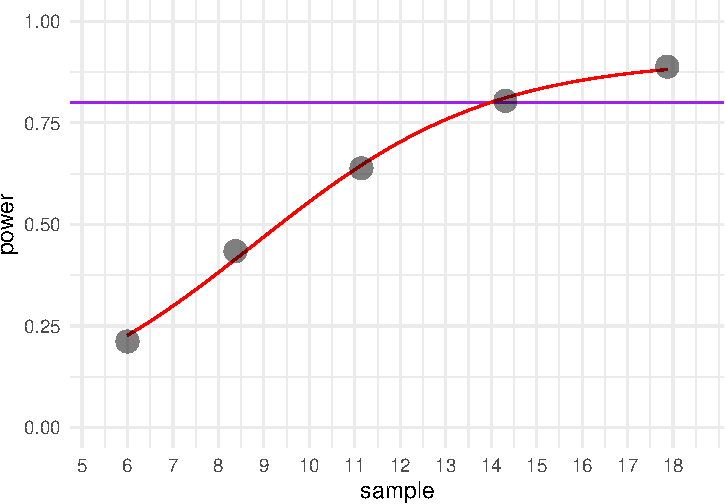
\includegraphics{PUMP_Manuscript_files/figure-latex/plotsamplepowercurve-1} \end{center}

\subsection{Comparing adjustment procedures}

It is easy to rerun the above using the Westfall-Young Stepdown
procedure (this procedure is much more computationally intensive to
run), or other procedures of interest. Alternatively, simply provide a
list of procedures you wish to compare. If you provide a list, the
package will re-run the power calculator for each item on the list; this
can make the overall call computationally intensive. Here we obtain
power for our scenario using Bonferroni, Holm and Westfall-Young
adjustments, and plot the results using the default \texttt{plot()}
method:

\begin{Shaded}
\begin{Highlighting}[]
\NormalTok{p2 \textless{}{-}}\StringTok{ }\KeywordTok{update}\NormalTok{( p\_check,}
              \DataTypeTok{MTP =} \KeywordTok{c}\NormalTok{(}\StringTok{"Bonferroni"}\NormalTok{, }\StringTok{"Holm"}\NormalTok{, }\StringTok{"WY{-}SD"}\NormalTok{),}
              \DataTypeTok{tnum =} \DecValTok{10000}\NormalTok{,}
              \DataTypeTok{parallel.WY.clusters =} \DecValTok{3}\NormalTok{ )}
\KeywordTok{plot}\NormalTok{( p2 )}
\end{Highlighting}
\end{Shaded}

\begin{center}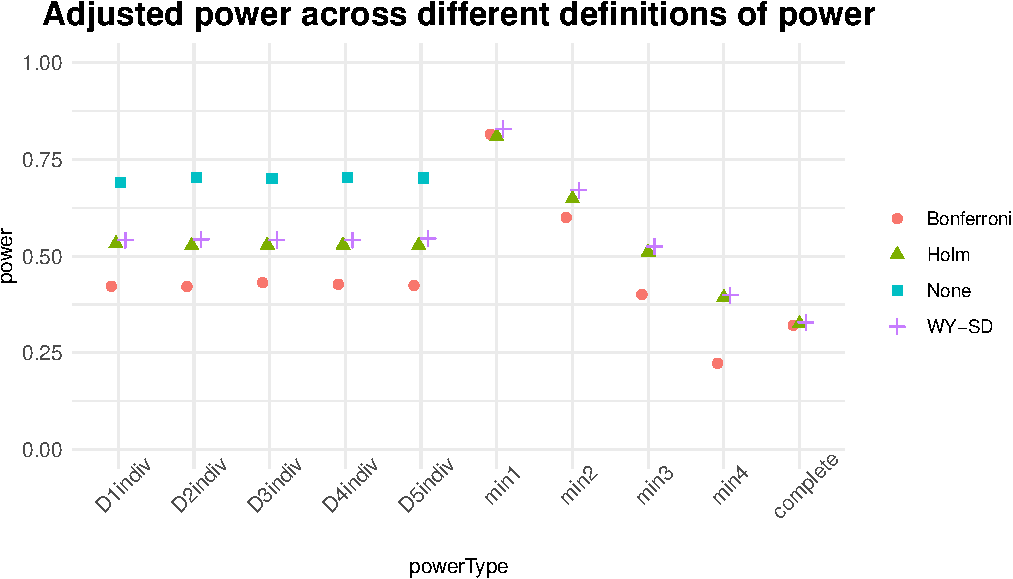
\includegraphics{PUMP_Manuscript_files/figure-latex/othercorrections-1} \end{center}

To speed up computation, we set \texttt{parallel.WY.clusters\ =\ 3} to
parallelize the computation. We also reduce \texttt{tnum} to decrease
computation time.

The more sophisticated (and less conservative) adjustment exploits the
correlation in our outcomes (\texttt{rho\ =\ 0.4}) to provide higher
individual power. Note, however, that we do not see elevated rates for
\(1-\)minimal power. Accounting for the correlation of the test
statistics when adjusting \(p\)-values can drive some power (individual
power) up, but on the flip side \(1-\)power can be driven down as the
lack of independence between tests gives fewer chances for a significant
result. See Porter (2018) for further discussion; while the paper
focuses on the multisite randomized trial context, the lessons learned
there apply to all designs as the only substantive differences between
different design and modeling choices is in how we calculate the
unadjusted distribution of their test statistics.

\subsection{Exploring sensitivity to design parameters}

Within the pump package we have two general ways of exploring design
sensitivity. The first is with \texttt{update()}, which allows for
quickly generating a single alternate scenario. To explore sensitivity
to different design parameters more systematically, use the
\texttt{grid()} functions, which calculate power, mdes, and sample size
for all combinations of a set of passed parameter values. There are two
main differences between the two approaches. First, \texttt{update()}
allows for different values of a parameter for the different outcomes;
the \texttt{grid} approach, by contrast, is more limited in this regard,
and assumes the same parameter value across different outcomes. Second,
the \texttt{grid} functions are a powerful tool for systematically
exploring many possible combinations, while \texttt{update()} only
allows the user to explore one value at a time.

We first illustrate the \texttt{update()} approach, and then turn to
illustrating \texttt{grid()} across three common areas of exploration:
Intraclass Correlation Coefficients (ICCs), the correlation of test
statistics, and the assumed number of non-zero effects. The last two are
particularly important for multiple outcome contexts.

\subsubsection{Exploring power with update()}

Update allows for a quick change of some of the set of parameters used
in a prior call; we saw \texttt{update()} used several times above. As a
further example, here we examine what happens if the ICCs are more
equally split across levels two and three:

\begin{Shaded}
\begin{Highlighting}[]
\NormalTok{p\_b \textless{}{-}}\StringTok{ }\KeywordTok{update}\NormalTok{( p\_check, }\DataTypeTok{ICC.2 =} \FloatTok{0.20}\NormalTok{, }\DataTypeTok{ICC.3 =} \FloatTok{0.25}\NormalTok{ )}
\KeywordTok{print}\NormalTok{( p\_b )}
\CommentTok{\#\textgreater{} power result: d3.2\_m3fc2rc design with 5 outcomes}
\CommentTok{\#\textgreater{}   MTP D1indiv D2indiv D3indiv D4indiv D5indiv indiv.mean    min1    min2}
\CommentTok{\#\textgreater{}  None 0.24513 0.24236 0.24333 0.24256 0.24491   0.243658      NA      NA}
\CommentTok{\#\textgreater{}  Holm 0.09800 0.09737 0.09711 0.09704 0.09799   0.097502 0.26677 0.11533}
\CommentTok{\#\textgreater{}     min3    min4 complete}
\CommentTok{\#\textgreater{}       NA      NA       NA}
\CommentTok{\#\textgreater{}  0.05815 0.03112  0.02399}
\CommentTok{\#\textgreater{}  0.000 \textless{}= SE \textless{}= 0.001}
\end{Highlighting}
\end{Shaded}

We immediately see that our assumption of substantial variation in level
three matters a great deal for power.

When calculating power for a given scenario, it is also easy to vary
many of our design parameters by outcome. For example, if we thought we
had better predictive covariates for our second outcome, we might try:

\begin{Shaded}
\begin{Highlighting}[]
\NormalTok{p\_d =}\StringTok{ }\KeywordTok{update}\NormalTok{( p\_check,}
            \DataTypeTok{R2.1 =} \KeywordTok{c}\NormalTok{( }\FloatTok{0.1}\NormalTok{, }\FloatTok{0.3}\NormalTok{, }\FloatTok{0.1}\NormalTok{, }\FloatTok{0.2}\NormalTok{, }\FloatTok{0.2}\NormalTok{ ),}
            \DataTypeTok{R2.2 =} \KeywordTok{c}\NormalTok{( }\FloatTok{0.4}\NormalTok{, }\FloatTok{0.8}\NormalTok{, }\FloatTok{0.3}\NormalTok{, }\FloatTok{0.2}\NormalTok{, }\FloatTok{0.2}\NormalTok{ ),}
            \DataTypeTok{omega.3 =} \KeywordTok{c}\NormalTok{( }\FloatTok{0.2}\NormalTok{, }\FloatTok{0.4}\NormalTok{, }\FloatTok{0.3}\NormalTok{, }\FloatTok{0.2}\NormalTok{, }\FloatTok{0.2}\NormalTok{ ) )}
\KeywordTok{print}\NormalTok{( p\_d )}
\CommentTok{\#\textgreater{} power result: d3.2\_m3fc2rc design with 5 outcomes}
\CommentTok{\#\textgreater{}   MTP D1indiv D2indiv D3indiv D4indiv D5indiv indiv.mean    min1    min2}
\CommentTok{\#\textgreater{}  None 0.43265 0.85325 0.38075 0.34358 0.34337   0.470720      NA      NA}
\CommentTok{\#\textgreater{}  Holm 0.24398 0.65388 0.21066 0.18851 0.18856   0.297118 0.71219 0.37367}
\CommentTok{\#\textgreater{}     min3    min4 complete}
\CommentTok{\#\textgreater{}       NA      NA       NA}
\CommentTok{\#\textgreater{}  0.21062 0.12208  0.08596}
\CommentTok{\#\textgreater{}  0.000 \textless{}= SE \textless{}= 0.001}
\end{Highlighting}
\end{Shaded}

Notice how the individual powers are heavily impacted. The \(d\)-minimal
powers naturally take the varying outcomes into account as we are
calculating a joint distribution of test statistics that will have the
correct marginal distributions based on these different design parameter
values.

After several \texttt{update()}s, we may lose track of where we are; to
find out, we can always check details with \texttt{print\_design()} or
\texttt{summary()}:

\begin{Shaded}
\begin{Highlighting}[]
\KeywordTok{summary}\NormalTok{(p\_d)}
\CommentTok{\#\textgreater{} power result: d3.2\_m3fc2rc design with 5 outcomes}
\CommentTok{\#\textgreater{}   MDES vector: 0.1, 0.1, 0.1, 0.1, 0.1}
\CommentTok{\#\textgreater{}   nbar: 258  J: 3    K: 15   Tbar: 0.5}
\CommentTok{\#\textgreater{}   alpha: 0.05    }
\CommentTok{\#\textgreater{}   Level:}
\CommentTok{\#\textgreater{}     1: R2: 0.1 / 0.3 / 0.1 / 0.2 / 0.2 (5 covariates)}
\CommentTok{\#\textgreater{}     2: R2: 0.4 / 0.8 / 0.3 / 0.2 / 0.2 (3 covariates)    ICC: 0.05   omega: 0}
\CommentTok{\#\textgreater{}     3:   fixed effects    rho = 0.4}
\CommentTok{\#\textgreater{}   MTP D1indiv D2indiv D3indiv D4indiv D5indiv indiv.mean    min1    min2}
\CommentTok{\#\textgreater{}  None 0.43265 0.85325 0.38075 0.34358 0.34337   0.470720      NA      NA}
\CommentTok{\#\textgreater{}  Holm 0.24398 0.65388 0.21066 0.18851 0.18856   0.297118 0.71219 0.37367}
\CommentTok{\#\textgreater{}     min3    min4 complete}
\CommentTok{\#\textgreater{}       NA      NA       NA}
\CommentTok{\#\textgreater{}  0.21062 0.12208  0.08596}
\CommentTok{\#\textgreater{}  0.000 \textless{}= SE \textless{}= 0.001}
\CommentTok{\#\textgreater{}  (tnum = 100000)}
\end{Highlighting}
\end{Shaded}

Using update allows for targeted comparison of major choices, but if we
are interested in how power changes across a range of options, we can do
this more systematically with the \texttt{grid()} functions, as we do
next.

\subsubsection{Exploring the impact of the ICC}

We above saw that the ICC does impact power considerably. We next extend
this evaluation by exploring a range of options for both level two and
three ICCs, so we can assess whether our power is sufficient across a
set of plausible values. The \texttt{update\_grid()} call makes this
straightforward: we pass our baseline scenario along with lists of
parameters to additionally explore:

\begin{Shaded}
\begin{Highlighting}[]
\NormalTok{grid \textless{}{-}}\StringTok{ }\KeywordTok{update\_grid}\NormalTok{( p\_check,}
            \DataTypeTok{ICC.2 =} \KeywordTok{seq}\NormalTok{( }\DecValTok{0}\NormalTok{, }\FloatTok{0.3}\NormalTok{, }\FloatTok{0.05}\NormalTok{ ),}
            \DataTypeTok{ICC.3 =} \KeywordTok{seq}\NormalTok{( }\DecValTok{0}\NormalTok{, }\FloatTok{0.60}\NormalTok{, }\FloatTok{0.20}\NormalTok{ ),}
            \DataTypeTok{tnum =} \DecValTok{5000}\NormalTok{ )}

\NormalTok{grid}\OperatorTok{$}\NormalTok{ICC}\FloatTok{.3}\NormalTok{ =}\StringTok{ }\KeywordTok{as.factor}\NormalTok{( grid}\OperatorTok{$}\NormalTok{ICC}\FloatTok{.3}\NormalTok{ )}
\NormalTok{grid =}\StringTok{ }\KeywordTok{filter}\NormalTok{( grid, MTP }\OperatorTok{==}\StringTok{ "Holm"}\NormalTok{ )}
\KeywordTok{ggplot}\NormalTok{( grid, }\KeywordTok{aes}\NormalTok{( ICC}\FloatTok{.2}\NormalTok{, min1, }\DataTypeTok{group =}\NormalTok{ ICC}\FloatTok{.3}\NormalTok{, }\DataTypeTok{col =}\NormalTok{ ICC}\FloatTok{.3}\NormalTok{ ) ) }\OperatorTok{+}
\StringTok{    }\KeywordTok{geom\_line}\NormalTok{() }\OperatorTok{+}\StringTok{ }\KeywordTok{geom\_point}\NormalTok{() }\OperatorTok{+}
\StringTok{    }\KeywordTok{labs}\NormalTok{( }\DataTypeTok{y =} \StringTok{"Min{-}1 Power"}\NormalTok{ ) }\OperatorTok{+}
\StringTok{  }\KeywordTok{coord\_cartesian}\NormalTok{( }\DataTypeTok{ylim=}\KeywordTok{c}\NormalTok{(}\DecValTok{0}\NormalTok{,}\DecValTok{1}\NormalTok{) )}
\end{Highlighting}
\end{Shaded}

\begin{center}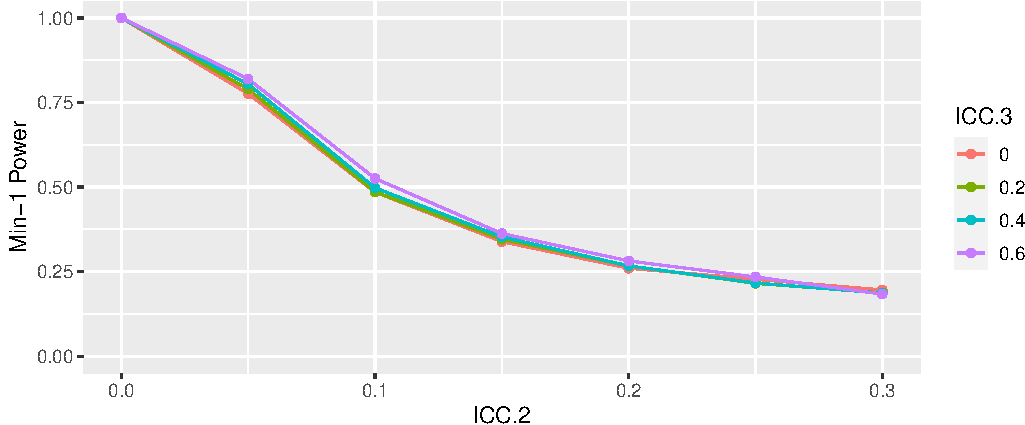
\includegraphics{PUMP_Manuscript_files/figure-latex/unnamed-chunk-8-1} \end{center}

\textcolor{red}{KH comment: maybe also demonstrate grid alone, in addition to update\_grid?}

We see that higher ICC.2 radically reduces power to detect anything and
ICC.3 does little. To understand why, we turn to our standard error
formula for this design and model: \[
\begin{aligned}
SE( \hat{\tau} ) = \sqrt{
\frac{\text{ICC}_{2}(1 - R^2_{2})}{\bar{T}(1 - \bar{T}) JK} +
\frac{(1-\text{ICC}_{2} - \text{ICC}_{3})(1-R^2_{1})}{\bar{T}(1 - \bar{T}) J K\bar{n}} } .
\end{aligned}
\] In the above, the \(\bar{n} = 258\) students per group makes the
second term very small compared to the first, regardless of the ICC.3
value. The first term, however, is a direct scaling of ICC.2; changing
it will change the standard error, and therefore power, a lot. All
provided designs and models implemented in the package are discussed,
along with corresponding formula such as these, in our technical
supplement accompanying this paper and package.

For grid searches we recommend reducing the number of permutations, via
\texttt{tnum}, to speed up computation. As \texttt{tnum} shrinks, we
will get increasingly rough estimates of power, but even these rough
estimates can help us determine trends.

The \texttt{grid()} functions provide easy and direct ways of exploring
how power changes as a function of the design parameters. We note,
however, that in order to keep syntax simple, they do not allow
different design parameters, including MDES, by outcome. This is to keep
package syntax simpler. When faced with contexts where it is believed
that these parameters do vary, we recommend using average values for the
broader searches, and then double-checking a small set of potential
final designs with the \texttt{pump\_power()} method.

\subsubsection{Exploring the impact of rho}

The correlation of test statistics, \(\rho\), is a critical parameter
for how power will play out across the multiple tests. For example, with
Westfall-Young, we saw that the correlation can improve our individual
power, as compared to Bonferroni. We might not know what will happen to
\(2-\)minimal power, however: on one hand, correlated statistics make
individual adjustment less severe, and on the other correlation means we
succeed or fail all together. We can explore this question relatively
easily by letting \texttt{rho} vary as so:

\begin{Shaded}
\begin{Highlighting}[]
\NormalTok{gridRho \textless{}{-}}\StringTok{ }\KeywordTok{update\_grid}\NormalTok{( p\_check,}
            \DataTypeTok{MTP =} \KeywordTok{c}\NormalTok{( }\StringTok{"Bonferroni"}\NormalTok{, }\StringTok{"WY{-}SD"}\NormalTok{ ),}
            \DataTypeTok{rho =} \KeywordTok{seq}\NormalTok{( }\DecValTok{0}\NormalTok{, }\FloatTok{0.9}\NormalTok{, }\DataTypeTok{by=}\FloatTok{0.15}\NormalTok{ ),}
            \DataTypeTok{tnum =} \DecValTok{500}\NormalTok{,}
            \DataTypeTok{B =} \DecValTok{10000}\NormalTok{ )}
\end{Highlighting}
\end{Shaded}

We then plot our results.

\begin{Shaded}
\begin{Highlighting}[]
\NormalTok{gridL =}\StringTok{ }\KeywordTok{filter}\NormalTok{( gridRho, MTP }\OperatorTok{!=}\StringTok{ "None"}\NormalTok{ ) }\OperatorTok{\%\textgreater{}\%}
\StringTok{  }\KeywordTok{pivot\_longer}\NormalTok{( }\DataTypeTok{cols =} \KeywordTok{c}\NormalTok{(indiv.mean, min1, min2, complete),}
                \DataTypeTok{names\_to =} \StringTok{"definition"}\NormalTok{, }\DataTypeTok{values\_to =} \StringTok{"power"}\NormalTok{ ) }\OperatorTok{\%\textgreater{}\%}
\StringTok{  }\KeywordTok{mutate}\NormalTok{( }\DataTypeTok{definition =} \KeywordTok{factor}\NormalTok{( definition,}
                            \DataTypeTok{levels =} \KeywordTok{c}\NormalTok{(}\StringTok{"indiv.mean"}\NormalTok{, }\StringTok{"min1"}\NormalTok{, }\StringTok{"min2"}\NormalTok{, }\StringTok{"complete"}\NormalTok{ ) ) )}

\KeywordTok{ggplot}\NormalTok{( gridL, }\KeywordTok{aes}\NormalTok{( rho, power, }\DataTypeTok{col=}\NormalTok{MTP ) ) }\OperatorTok{+}
\StringTok{  }\KeywordTok{facet\_grid}\NormalTok{( . }\OperatorTok{\textasciitilde{}}\StringTok{ }\NormalTok{definition ) }\OperatorTok{+}
\StringTok{  }\KeywordTok{geom\_line}\NormalTok{() }\OperatorTok{+}\StringTok{ }\KeywordTok{geom\_point}\NormalTok{() }\OperatorTok{+}
\StringTok{  }\KeywordTok{geom\_hline}\NormalTok{( }\DataTypeTok{yintercept =} \KeywordTok{c}\NormalTok{( }\DecValTok{0}\NormalTok{, }\FloatTok{0.80}\NormalTok{ ) ) }\OperatorTok{+}\StringTok{ }
\StringTok{  }\KeywordTok{theme\_minimal}\NormalTok{() }\OperatorTok{+}
\StringTok{  }\KeywordTok{coord\_cartesian}\NormalTok{( }\DataTypeTok{ylim=}\KeywordTok{c}\NormalTok{(}\DecValTok{0}\NormalTok{,}\DecValTok{1}\NormalTok{) )}
\end{Highlighting}
\end{Shaded}

\begin{center}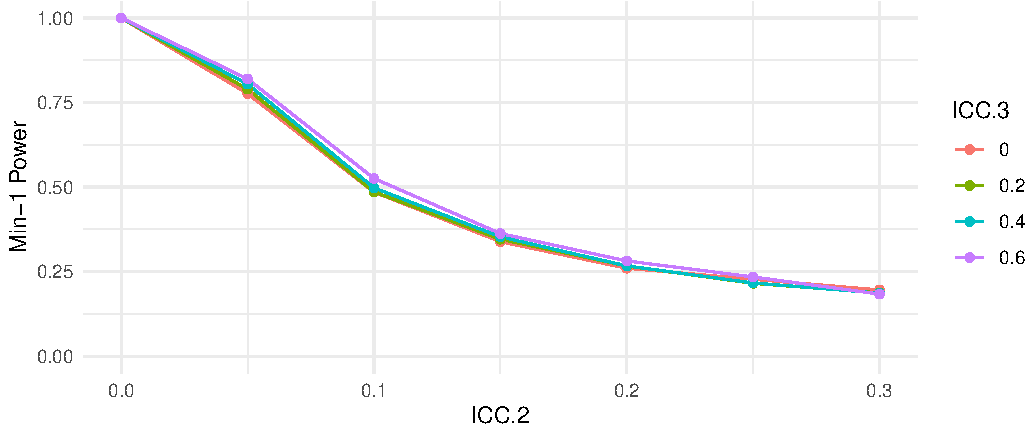
\includegraphics{PUMP_Manuscript_files/figure-latex/unnamed-chunk-11-1} \end{center}

First, we see the benefit of the Westfall-Young single-step procedure is
minimal, as compared to Bonferroni. Second, the impact on individual
adjustment is flat, as anticipated. Third, across a very broad range of
rho, we maintain good \(1-\)minimal power. Complete power climbs as
correlation increases, and \(2-\)minimal power is generally unchanged.

\subsubsection{Exploring the impact of null outcomes}

We finally explore varying the number of outcomes with no effects. This
exploration is an important way to hedge a design against the
possibility that some number of the identified outcomes are measured
poorly, or are simply not impacted by treatment. We use a grid search,
varying the number of outcomes that have no treatment impact via the
\texttt{numZero} design parameter:

\begin{Shaded}
\begin{Highlighting}[]
\NormalTok{gridZero \textless{}{-}}\StringTok{ }\KeywordTok{update\_grid}\NormalTok{( p\_check,}
            \DataTypeTok{numZero =} \DecValTok{0}\OperatorTok{:}\DecValTok{4}\NormalTok{,}
            \DataTypeTok{M =} \DecValTok{5}\NormalTok{ )}
\end{Highlighting}
\end{Shaded}

We then can make a plot as we did above:

\begin{center}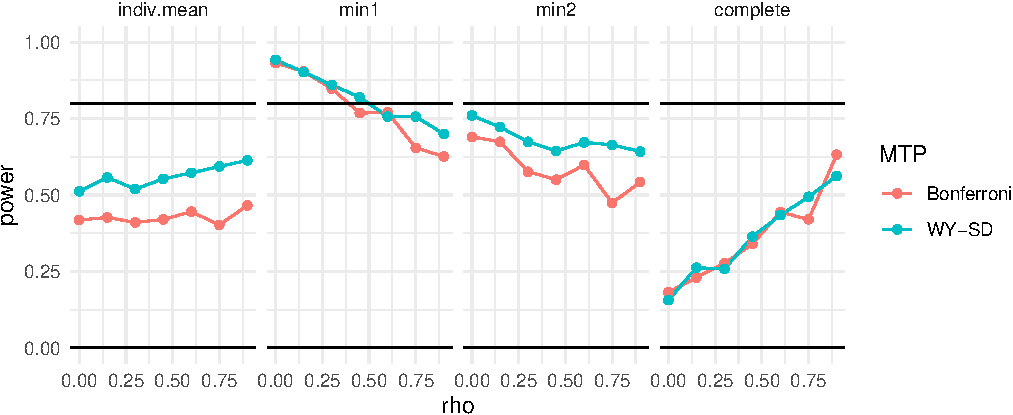
\includegraphics{PUMP_Manuscript_files/figure-latex/unnamed-chunk-14-1} \end{center}

There are other ways of exploring the impact of weak or null effects on
some outcomes. In particular, the \texttt{pump\_power()} and
\texttt{pump\_sample()} methods allow the researcher to provide an MDES
vector with different values for each outcome, including 0s for some
outcomes. The \texttt{grid()} functions, by contrast, take a single MDES
value for the non-null outcomes, with a separate specification of how
many of the outcomes are 0. (This single value plus \texttt{numZero}
parameter also works with \texttt{pump\_power()} if desired.)

\section{Conclusion}
\label{sec:conclusion}

We introduce the power under multiplicity project (\texttt{PUMP})
\texttt{R} package, which estimates power for multi-level randomized
control trials with multiple outcomes. \texttt{PUMP} allows users to
estimate power, MDES, and sample size requirements for a wide variety of
commonly used RCT designs and models across different definitions of
power and applying different MTPs. The functionality of \texttt{PUMP}
fills an important gap, as existing tools do not allow researchers to
conduct power, MDES or sample size calculations when applying a MTP.

The main advantage of the \texttt{PUMP} package is to provide easily
accessible estimation procedures so that users can properly account for
power when making adjustments for multiple hypothesis testing. Users can
also take advantage of the \texttt{PUMP} in an online interface at
www.mdrcpump.io. However, one of the additional strengths of the package
is the ease with which a user can explore the impact of different
designs, models, and assumptions on power, MDES or sample size. Even if
a user is only interested in a single outcome, \texttt{PUMP} provides
useful functionality for more robust power calculations. A user can and
should try a range of parameter values to determine the sensitivity of
the power of their study to different assumptions; this package
simplifies that process.

\section*{Acknowledgements}

We acknowledge the Diplomas Now team at MDRC. Development of this
package was supported by a grant from the Institute for Education
Sciences (R305D170030). We would like to thank members of the Harvard
CARES lab for their feedback on the manuscript.

\section{References}

\hypertarget{refs}{}
\begin{cslreferences}
\leavevmode\hypertarget{ref-RN33089}{}%
Bang, Jung, H. 2005. ``Sample Size Calculation for Simulation-Based
Mulitple-Testing Procedures.'' Journal Article. \emph{Journal of
Biopharmaceutical Statistics} 15: 957--67.

\leavevmode\hypertarget{ref-lme4}{}%
Bates, Douglas, Martin Mächler, Ben Bolker, and Steve Walker. 2015.
``Fitting Linear Mixed-Effects Models Using lme4.'' \emph{Journal of
Statistical Software} 67 (1): 1--48.
\url{https://doi.org/10.18637/jss.v067.i01}.

\leavevmode\hypertarget{ref-BenjaminiHochberg1995}{}%
Benjamini, \& Hochberg, Y. 1995. ``Controlling the False Discovery Rate:
A Practical and Powerful Approach to Multiple Testing.'' \emph{Journal
of the Royal Statistical Society: Series B} 57 (1): 289--300.

\leavevmode\hypertarget{ref-RN27978}{}%
Bloom, Howard S. 2006. ``The Core Analytics of Randomized Experiments
for Social Research.'' Government Document. MDRC.

\leavevmode\hypertarget{ref-RN23882}{}%
Chen, Luo, J. 2011. ``On Power and Sample Size Computation for Multiple
Testing Procedures.'' Journal Article. \emph{Computational Statistics
and Data Analysis} 55: 110--22.

\leavevmode\hypertarget{ref-DNREPORT}{}%
Corrin W., Rosen, Sepanik S. 2016. ``Addressing Early Warning
Indicators: Interim Impact Findings from the Investing in Innovation
(I3) Evaluation of Diplomas Now.'' Government Document. MDRC.

\leavevmode\hypertarget{ref-RN4473}{}%
Dong, Nianbo, and Rebecca Maynard. 2013. ``PowerUP!: A Tool for
Calculating Minimum Detectable Effect Sizes and Minimum Required Sample
Sizes for Experimental and Quasi-Experimental Design Studies.'' Journal
Article. \emph{Journal of Research on Educational Effectiveness} 6 (1):
24--67.

\leavevmode\hypertarget{ref-RN23878}{}%
Dudoit, Shaffer, S. 2003. ``Multiple Hypothesis Testing in Microarray
Experiments.'' Journal Article. \emph{Statistical Science} 18 (1):
71--103.

\leavevmode\hypertarget{ref-RN24280}{}%
Dunn, Olive Jean. 1959. ``Estimation of the Medians for Dependent
Variables.'' Journal Article, 192--97.
\url{https://doi.org/10.1214/aoms/1177706374}.

\leavevmode\hypertarget{ref-RN24281}{}%
---------. 1961. ``Multiple Comparisons Among Means.'' Journal Article.
\emph{Journal of the American Statistical Association} 56 (293): 52--64.
\url{https://doi.org/10.1080/01621459.1961.10482090}.

\leavevmode\hypertarget{ref-RN30153}{}%
Hedges, Larry V., and Christopher Rhoads. 2010. ``Statistical Power
Analysis in Education Research.'' Report. National Center for Special
Education Research.
\url{http://www.eric.ed.gov/ERICWebPortal/detail?accno=ED509387}.

\leavevmode\hypertarget{ref-RN24282}{}%
Holm, S. 1979. ``A Simple Sequentially Rejective Multiple Test
Procedure.'' Journal Article. \emph{Scand. J. Statist.} 6 (2): 65--70.

\leavevmode\hypertarget{ref-Porter2018}{}%
Porter, Kristin E. 2018. ``Statistical Power in Evaluations That
Investigate Effects on Multiple Outcomes: A Guide for Researchers.''
Journal Article. \emph{Journal of Research on Educational Effectiveness}
11 (2): 267--95.

\leavevmode\hypertarget{ref-RN23884}{}%
Raudenbush, S. W., J. Spybrook, R. Congdon, X. Liu, A. Martinez, H.
Bloom, and C Hill. 2011. ``Optimal Design Plus Empirical Evidence
(Version 3.0).'' Report.
\url{http://wtgrantfoundation.org/resource/optimal-design-with-empirical-information-od}.

\leavevmode\hypertarget{ref-RN23748}{}%
Schochet, Peter Z. 2008. ``Guidelines for Multiple Testing in Impact
Evaluations of Educational Interventions. Final Report.'' Report.
Mathematica Policy Research, Inc. P.O. Box 2393, Princeton, NJ
08543-2393.
\url{http://www.eric.ed.gov/ERICWebPortal/contentdelivery/servlet/ERICServlet?accno=ED502199}.

\leavevmode\hypertarget{ref-RN23881}{}%
Senn, Stephen, and Frank Bretz. 2007. ``Power and Sample Size When
Multiple Endpoints Are Considered.'' Journal Article.
\emph{Pharmaceutical Statistics} 6: 161--70.
\url{https://doi.org/10.1002/pst.301}.

\leavevmode\hypertarget{ref-RN352}{}%
Shaffer, Juliet Popper. 1995. ``Multiple Hypothesis Testing.'' Journal
Article. \emph{Annual Review of Psychology} 46 (1): 561--84.

\leavevmode\hypertarget{ref-RN24179}{}%
Spybrook, Jessica, H. S. Bloom, Richard Congdon, Carolyn J. Hill, Andres
Martinez, and Stephen W. Raudenbush. 2011. ``Optimal Design Plus
Empirical Evidence: Documentation for the `Optimal Design' Software
Version 3.0.'' Report.
\url{http://wtgrantfoundation.org/resource/optimal-design-with-empirical-information-od}.

\leavevmode\hypertarget{ref-RN33098}{}%
Tukey, J. W. 1953. ``The Problem of Multiple Comparisions.'' Report.
Princeton University.

\leavevmode\hypertarget{ref-RN28696}{}%
Westfall, Peter H, and S Stanley Young. 1993. \emph{Resampling-Based
Multiple Testing: Examples and Methods for P-Value Adjustment}. Book.
Vol. 279. John Wiley \& Sons.

\leavevmode\hypertarget{ref-MTSAS}{}%
Westfall, Tobias, Peter H, and R. D. Wolfinger. 2011. \emph{Multiple
Comparisons and Multiple Tests Using Sas}. Book. The SAS Institute.
\end{cslreferences}

\section{Appendix: Validation}

In order to validate that our power estimates are working as intended,
we compared three different methods of estimating power:

\begin{itemize}
\tightlist
\item
  \texttt{PUMP}
\item
  \texttt{PowerUpR}
\item
  Monte Carlo simulations
\end{itemize}

We compute values from \texttt{PowerUpR} for individual, unadjusted
power, as \texttt{PowerUpR} only provides power estimates in that
setting. For all other types of power definitions and adjustments, we
are only able to compare \texttt{PUMP} to the estimated power from Monte
Carlo simulations. We follow the simulation approach outlined in detail
in Section\textasciitilde{}\ref{sec:est_power}. After repeatedly
simulating data and calculating \(p\)-values, we calculate power and a
95\% confidence interval, assuming a conservative standard error
estimate of \(\sqrt{0.25/S}\).

To validate the estimates, we first check that the \texttt{PUMP} and
\texttt{PowerUpR} estimates match. In some settings we expect some
discrepancies between these values because \texttt{PUMP} has different
assumptions than \texttt{PowerUpR} for certain models. For details about
differences between \texttt{PUMP} and \texttt{PowerUpR} assumptions, see
the Supplementary Materials. Second, we check that the \texttt{PUMP}
estimate is within the Monte Carlo confidence interval.

We also validate MDES and sample size calculations. For MDES, we choose
one default scenario for each design and model, then input the
already-calculated individual power and see if the output MDES is the
same as the original input MDES. Similarly, for sample size validation,
we input the already-calculated individual power and see if the output
sample size (\texttt{nbar}, \texttt{J}, and \texttt{K} depending on
design) is the same as the original input sample size.

\textbf{Simulation parameters}

In order to validate that the method works in a wide range of scenarios,
which vary the following parameters.

Parameters that vary:

\begin{tabular}{l l l}
Parameter               & Default                & Comparison values \\ \hline
school size $\bar{n}$   & 50                     & 75, 100           \\
$R^2$                   & 0                      & 0.6               \\
$\rho$                  & 0.5                    & 0.2, 0.8          \\
MDES                    & (0.125, 0.125, 0.125)  & (0.125, 0, 0)     \\
ICC                     & 0.2                    & 0.7               \\
$\omega$                & 0.1                    & 0.8               \\
\end{tabular}

We do not vary:

\begin{itemize}
\tightlist
\item
  \texttt{M\ =\ 3}
\item
  \texttt{J} and \texttt{K} are fixed for each scenario
\item
  Scalar grand mean of control outcomes
\item
  Correlations between school random effects and impacts
\item
  \texttt{rho} informs all correlations; we keep the same correlation
  between covariates, residuals, impacts, random effects for all levels
  and across all outcomes
\end{itemize}

\textbf{Validation results}

Below is an example of a graph we use for validation. The green dots are
\texttt{PUMP} estimate of power, the red dot is the \texttt{PowerUpR}
estimate of power, and the 95\% confidence intervals based on the Monte
Carlo simulations are shown in blue. To validate that \texttt{PUMP}
produces the expected result, we want to see the red and green points
match, and for the red point to be within the blue intervals.
Figure\textasciitilde{}\ref{fig:validate} shows the results across
different types of power and different MTPs. We repeat this plot for a
variety of different parameter values for each design and model.

\begin{figure}
  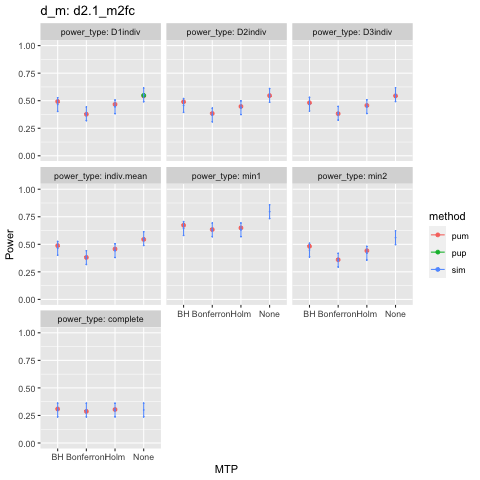
\includegraphics[width=\linewidth]{example_validation_plot.png}
  \label{fig:validate}
\end{figure}

Next, we validate MDES and sample size calculations. We put in our found
power, and then see if the \texttt{pump\_mdes()} function returns the
MDES we originally plugged in to achieve this power. In
Table\textasciitilde{}\ref{tab:mdes}, the first column shows the
calculated MDES, the middle column is the power we plugged into the
calculation, and the last column shows the MDES that we are targeting.
Thus, ideally we want the first and last columns to match.

\begin{table}
\centering
\begin{tabular}{lrrr}
MTP & Adjusted MDES & D1indiv Power & Target MDES\\
\hline
Bonferroni & 0.122 & 0.447 & 0.125\\
BH & 0.127 & 0.578 & 0.125\\
Holm & 0.125 & 0.540 & 0.125
\end{tabular}
\label{tab:mdes}
\end{table}

Similarly, we validate our sample size calculations. Using our found
power, we see if \texttt{pump\_sample()} returns the original sample
size. In Table\textasciitilde{}\ref{tab:ss}, we are targeting a sample
size of \(J = 20\).

\begin{table}
\centering
\begin{tabular}{llrr}
MTP & Sample.type & Sample.size & D1indiv.power\\
\hline
Bonferroni & J & 21 & 0.500\\
BH & J & 21 & 0.580\\
Holm & J & 20 & 0.544
\end{tabular}
\label{tab:ss}
\end{table}

\end{document}
